\documentclass[a5paper]{article}
\usepackage[a5paper, top=8mm, bottom=8mm, left=8mm, right=8mm]{geometry}

\usepackage{polyglossia}
\setdefaultlanguage[babelshorthands=true]{russian}

\usepackage{fontspec}
\setmainfont{FreeSerif}
\newfontfamily{\russianfonttt}[Scale=0.7]{DejaVuSansMono}

\usepackage[font=scriptsize]{caption}

\usepackage{amsmath}
\usepackage{amssymb,amsfonts,textcomp}
\usepackage{color}
\usepackage{array}
\usepackage{hhline}
\usepackage{cite}

\usepackage[hang,multiple]{footmisc}
\renewcommand{\footnotelayout}{\raggedright}

\PassOptionsToPackage{hyphens}{url}\usepackage[xetex,linktocpage=true,plainpages=false,pdfpagelabels=false]{hyperref}
\hypersetup{colorlinks=true, linkcolor=blue, citecolor=blue, filecolor=blue, urlcolor=blue, pdftitle=1, pdfauthor=, pdfsubject=, pdfkeywords=}

\usepackage{tabu}

\usepackage{graphicx}
\usepackage{indentfirst}
\usepackage{multirow}
\usepackage{subfig}
\usepackage{footnote}
\usepackage{minted}

\sloppy
\pagestyle{plain}

\title{Лекция 15: Примеры архитектур}
\author{Юрий Литвинов\\\small{y.litvinov@spbu.ru}}
\date{15.12.2022}

\begin{document}

\maketitle
\thispagestyle{empty}

\section{Введение}

В этой лекции мы рассмотрим примеры архитектур разных приложений из совершенно разных предметных областей, одно даже шуточное, но довольно поучительное. Начать имеет смысл с первоисточников, по которым подготовлена эта лекция:
\begin{itemize}
    \item репозиторий Enterprise Fizz-Buzz: \url{https://github.com/EnterpriseQualityCoding/FizzBuzzEnterpriseEdition};
    \item обзор архитектуры Bash в <<The Architecture of Open Source Applications>>\footnote{Глава про Bash в AOSA: \url{http://aosabook.org/en/bash.html} (дата обращения: 10.12.2020)}, правда про Bash из J. Garcia et al., <<Obtaining Ground-Truth Software Architectures>>\footnote{Публикация на IEEE Xplore: \url{https://ieeexplore.ieee.org/document/6606639} (дата обращения: 10.12.2020)};
    \item краткий обзор архитектуры Git в той же <<The Architecture of Open Source Applications>>\footnote{Глава про Git в AOSA: \url{http://aosabook.org/en/git.html} (дата обращения: 10.12.2020)} и, что полезнее, но длиннее, глава 10 Git Book\footnote{Git Book: \url{https://git-scm.com/book} (дата обращения: 10.12.2020)};
    \item обзор архитектуры Battle for Wesnoth снова из <<The Architecture of Open Source Applications>>\footnote{Глава про Battle for Wesnoth в AOSA: \url{http://aosabook.org/en/wesnoth.html} (дата обращения: 10.12.2020)}.
\end{itemize}

\section{Enterprise Fizz-Buzz}

 Начнём мы с самого серьёзного реального приложения --- FizzBuzz Enterprise Edition, созданного серьёзными бизнесменами для серьёзных бизнес-задач. Проект, естественно, сатира, высмеивающая безумные практики enterprise-программирования в Java-мире, но нам будет полезна как пример овердизайна. Мне кажется, проще понять, что такое хорошая архитектура, если на одном конце шкалы будет один большой класс, который всё делает, а на другом --- FizzBuzz Enterprise Edition с его подсистемой возврата перевода строки и прочими интересными архитектурными решениями. К тому же, там на самом деле используются (разумеется, не по делу) паттерны и архитектурные приёмы, которые были в этом курсе.

Собственно, серьёзная бизнес-задача такая:

Для чисел от 1 до 100:
\begin{itemize}
    \item если число делится на 3, вывести <<Fizz>>;
    \item если число делится на 5, вывести <<Buzz>>;
    \item если число делится и на 3, и на 5, вывести <<FizzBuzz>>;
    \item во всех остальных случаях вывести само число.
\end{itemize}

<<Правильное>> архитектурное решение можно найти тут: \url{https://github.com/EnterpriseQualityCoding/FizzBuzzEnterpriseEdition}.

\subsection{Обзор архитектуры}

Вот обзорная диаграмма, описывающая в общих чертах структуру этого проекта:

\begin{center}
    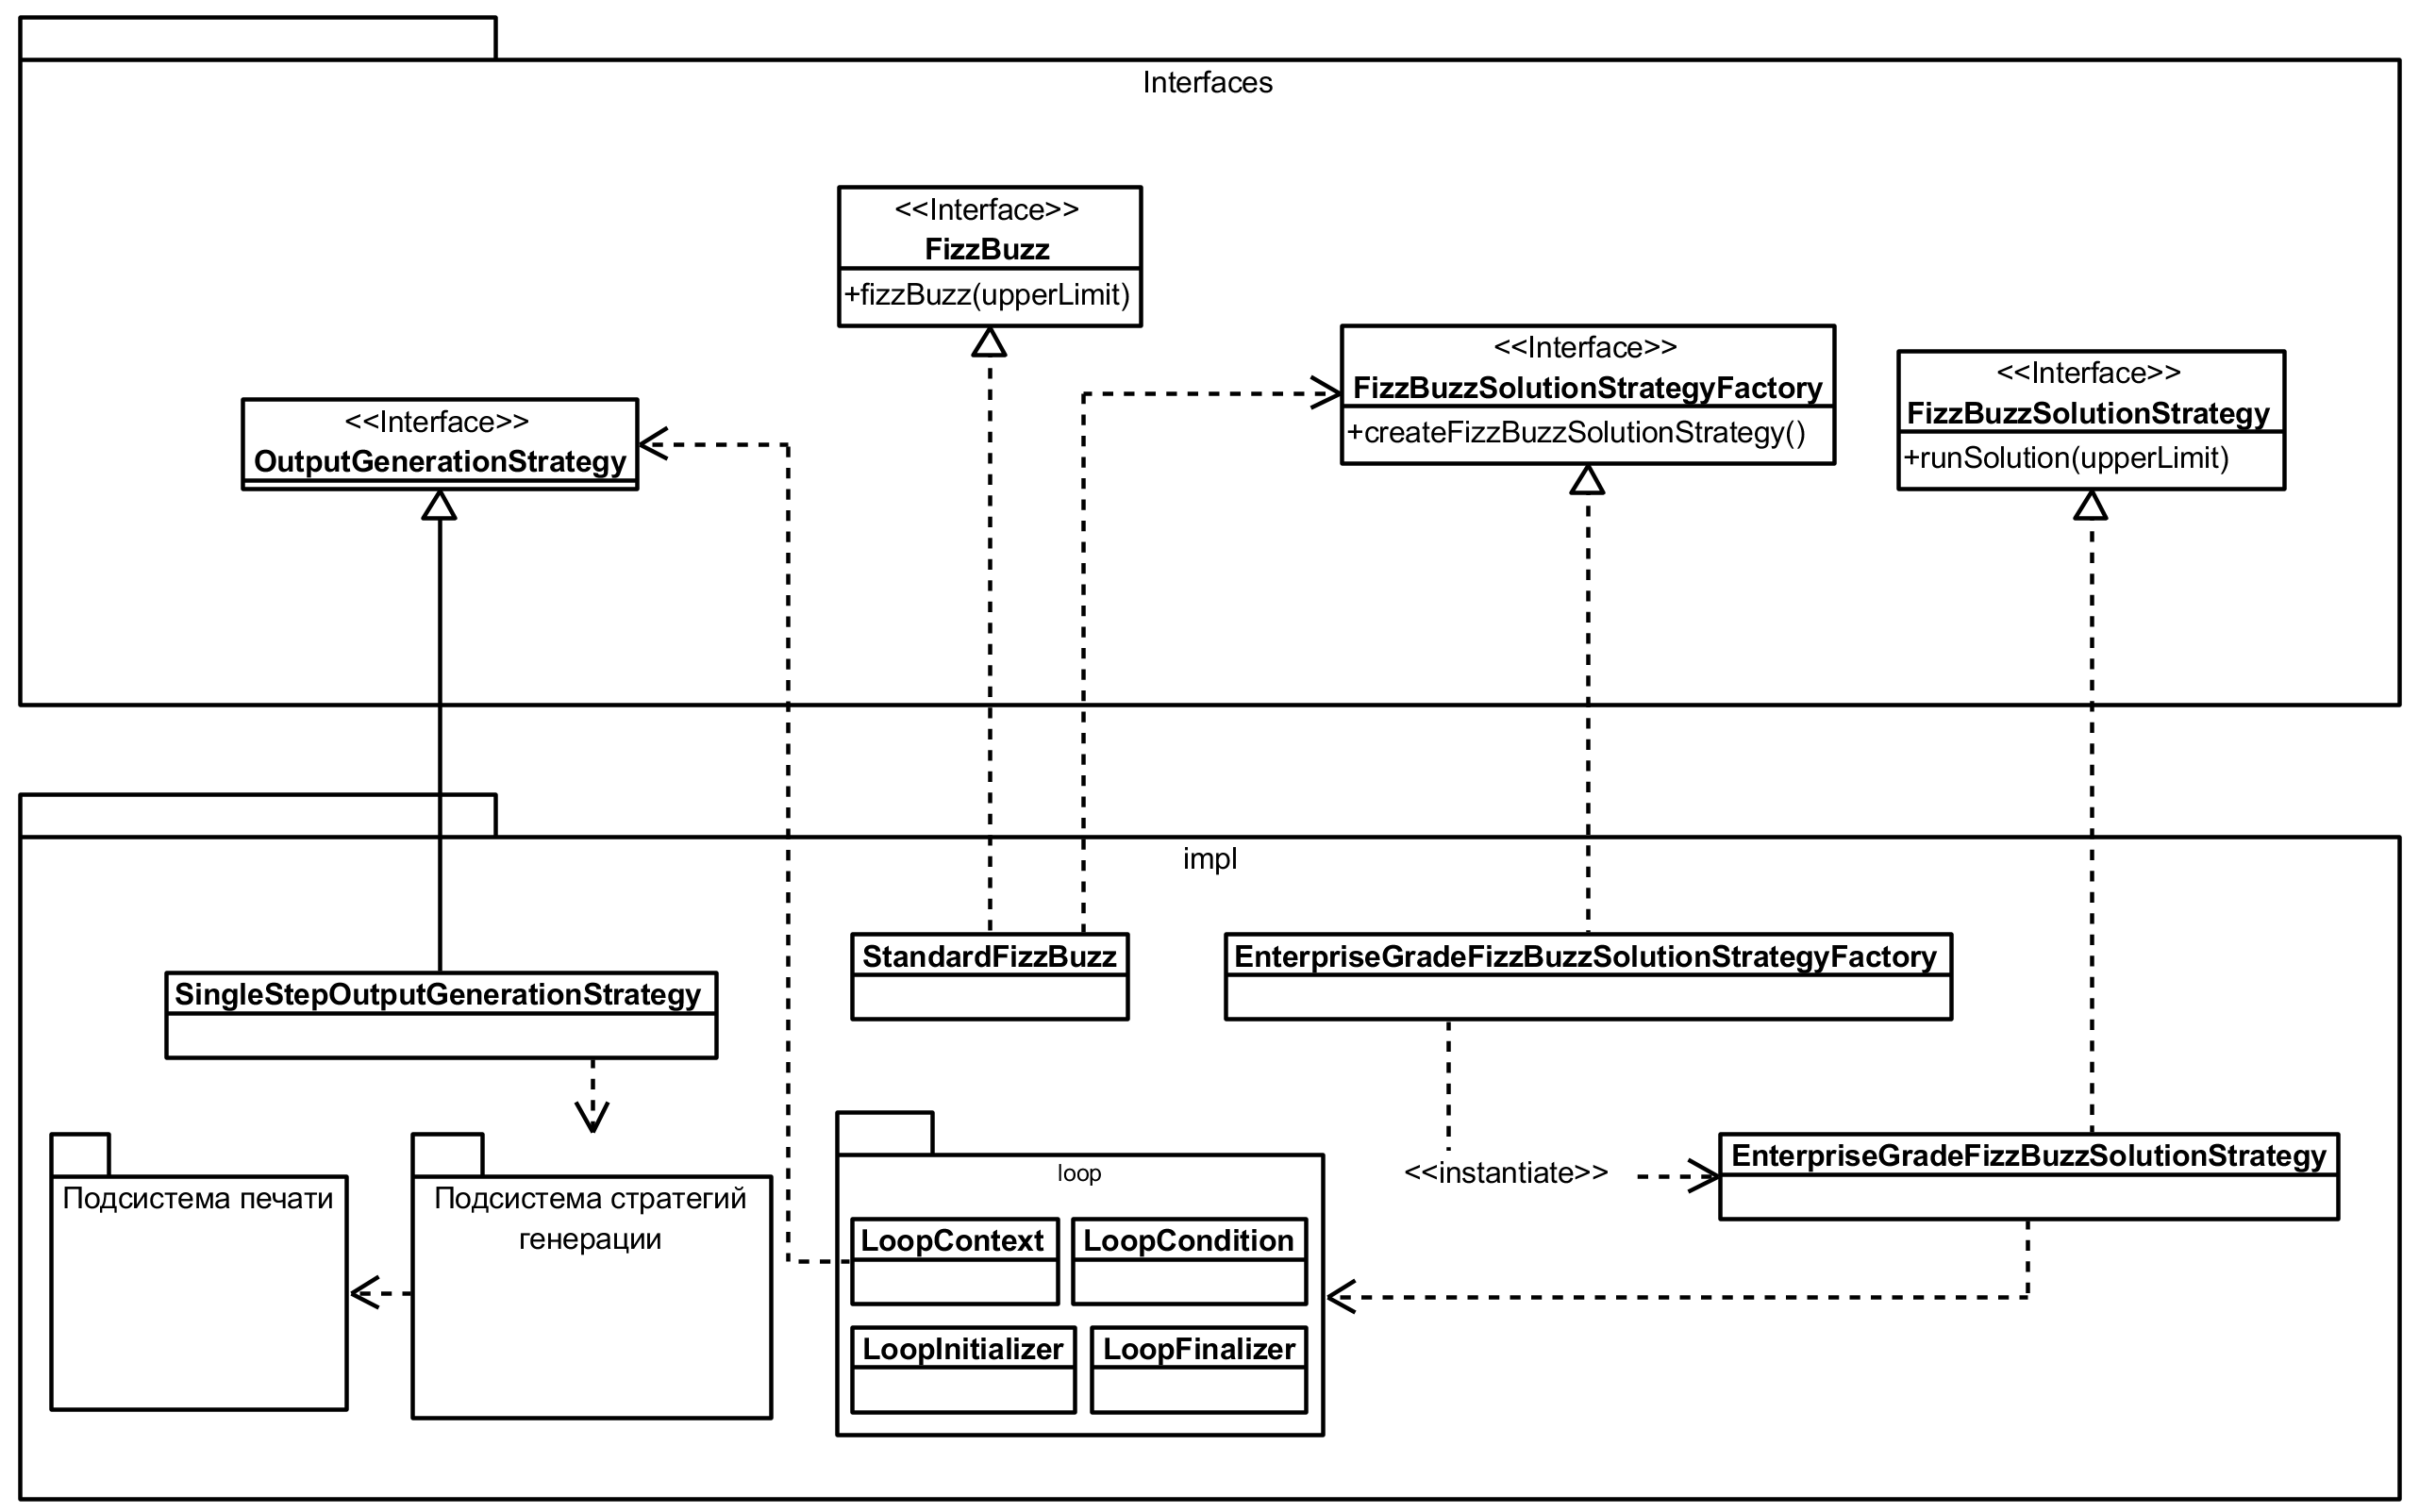
\includegraphics[width=\textwidth]{fizzBuzzArchitecture.png}
\end{center}

По данным OpenHub.net, реализация на момент анализа проекта содержала 1662 содержательные строки кода и очень немного комментариев. OpenHub.net оценивает стоимость разработки этого проекта в 18К долларов.

Собственно, как всё работает: main создаёт ApplicationContext --- класс из Spring Framework, который строит систему из доступных классов, используя принцип Dependency Injection. Общая идея Dependency Injection состоит в том, что процесс создания объектов, их сборки и инициализации сложной системы --- отдельная большая подзадача, которую не стоит делать прямо в <<боевом>> коде, иначе нарушится принцип единственности ответственности. Правильнее автоматизировать этот процесс, описав набор интерфейсов, использовав эти интерфейсы в <<боевых>> классах, а затем доверив сторонней библиотеке (в нашем случае, Spring) пройтись рефлексией по нашей кодовой базе и каждому, кто в конструктор принимает объект некоторого интерфейса, автоматически подставить созданный объект класса, реализующего этот интерфейс.

Сама логика работы реализуется классом StandardFizzBuzz, который сам решать задачу не умеет, но умеет создать стратегию решения (через фабрику стратегий, потому что он не хочет знать о конкретном классе-стратегии). Стратегия создаёт подсистему управления циклом (ну раз в условии написано про числа от 1 до 100), подсистема состоит из классов, отвечающих за границы цикла, условие завершения, и главное, действия, выполняемые на каждом шаге цикла. Ещё есть хранилище текущего контекста вычисления цикла, хранящее счётчик цикла, такие дела.

Механизм вычисления одного шага цикла тоже использует паттерн <<Стратегия>> --- сам он не хочет ничего считать, но делегирует вычисление стратегии генерации вывода. Стратегия генерации вывода принимает выходные данные, которые соответствуют счётчику цикла, но она не хочет знать про хранилище состояния цикла, в котором эти данные находятся, поэтому применяется адаптер (класс со звучным названием LoopContextStateRetrievalToSingleStepOutputGenerationAdapter), роль которого состоит в конвертации контекста цикла в параметр стратегии генерации. А вот стратегия генерации содержит в себе три стратегии вычисления, лежащие в одном списке, и для каждого значения счётчика цикла передаёт это значение всем этим трём стратегиям. Эти стратегии --- FizzStrategy, BuzzStrategy и NoFizzNoBuzzStrategy, которые про параметр цикла говорят, надо с ним что-то делать или нет (так что на самом деле это паттерн <<Спецификация>>, хотя в коде он так не называется --- стратегии сами ничего не делают). Стратегии определяют, можно ли печатать Fizz, Buzz или FizzBuzz, после чего вызывается подсистема генерации, которая и печатает строку на экран.

\subsection{Чему можно научиться}

Положительные стороны этого решения такие.
\begin{itemize}
    \item Separation of Concerns --- один класс решает строго одну задачу, при этом для каждой задачи из предметной области можно указать класс, который ей занимается. Это хорошо, потому что если что-то изменится в условии, надо будет менять, скорее всего, вполне конкретный класс, результаты изменения будет легко проверить юнит-тестами (ну, по идее, в этом проекте с юнит-тестами беда). Это же способствует переиспользованию кода и вообще сопровождаемости программы ---- из маленьких кирпичиков легко собрать новую программу в той же области, чем пытаться пилить под свои задачи большие куски кода.
    \item Dependency Inversion --- реализация не должна зависеть от другой реализации, обе они должны зависеть от абстракции. В этом проекте почти никто не знает о других классах, есть чётко описанные интерфейсы, и класс может только вызывать методы по интерфейсу. Почему это хорошо --- резко снижается связность. Не важно, как реализован тот или иной интерфейс --- пока есть реализация всех нужных ему интерфейсов, наш класс будет работать. Мы можем дописывать новые реализации, изменять старые, пробовать разные реализации и даже выбирать их в зависимости от ситуации --- при этом придётся переписывать минимум кода.
    \item Dependency Injection --- становится возможным благодаря активному применению принципа Dependency Inversion. Мы можем динамически создавать и вставлять реализации интерфейсов в классы, которым эти реализации нужны. При этом используется сторонняя библиотека Spring Framework, что тоже хорошая идея --- неспецифичные для предметной области задачи, скорее всего, уже давно решены, и лучше, чем вы когда-либо сделаете.
    \item Паттерны:
    \begin{itemize}
        \item <<Фабрика>> --- для создания объектов, реализующих интерфейсы, позволяет легко менять реализацию и отделяет использование от создания;
        \item <<Стратегия>> --- инкапсулирует алгоритм работы, позволяет легко менять алгоритмы;
        \item <<Посетитель>> --- тут не особо нужен, но вообще позволяет отделить логику обхода структуры данных, состоящих из нескольких классов, от действий, выполняемых при обходе; 
        \item <<Адаптер>> --- чтобы объект, реализующий один интерфейс, мог использоваться объектом, ожидающим другой интерфейс; опять-таки, уменьшает связность системы;
        \item <<Спецификация>> --- инкапсулирует сложное логическое условие или запрос; тут используется, чтобы определиться, когда что печатать;
        \item <<Цепочка ответственности>> --- позволяет сделать список (или воообще как-то организовать цепочку) объектов, каждый из которых может обработать запрос, либо отдать дальше, если не может; тут это не совсем <<Цепочка ответственности>>, потому что запрос может быть обработан двумя стратегиями сразу.
    \end{itemize}
\end{itemize}

\subsection{Почему если бы это была домашка, она была бы не зачтена}

\begin{itemize}
    \item Не выполняется принцип Keep It Simple Stupid. Хорошее решение должно быть максимально простым из тех, что всё ещё решают задачу \textbf{и} способны внятно объяснить способ её решения. Чем сложнее решение, тем сложнее его понять и, соответственно, сопровождать. Закладывать в архитектуру что-либо <<на будущее>> надо с умом, потому что, как правило, будущее так и не наступает (или наступает, но другое), а за это надо платить сложностью
    \begin{itemize}
        \item Кстати, какой-то достойный человек (жаль не помню кто) говорил <<Неправильно говорить ``строк кода написано'', правильно --- ``строк кода израсходовано'' на решение той или иной задачи>>. Производительность труда программиста глупо мерять количеством строк кода, потому что из двух решений одной задачи лучше то, которое короче и проще. То есть лучше тот программист, который по традиционным метрикам работает хуже. Однако это не значит, что код лучше вообще не писать, или, тем более, писать всё в одну строку, используя только однобуквенные идентификаторы --- \textit{объясняющая способность программы} важнее её размера. Программа как книга --- некоторые были бы лучше, если бы были короче (как EnterpriseFizzBuzz), некоторые были бы лучше, если бы были длиннее (как многие олимпиадные решения).
    \end{itemize}
    \item <<Синтаксическое>> разделение на пакеты, а не <<семантическое>>. Есть пакет interfaces, есть пакет adapters и т.д. Мне как читателю программы такое разбиение на пакеты ничего не говорит, я и так вижу, что там, например, одни интерфейсы. А вот то, что классы, отвечающие за определение, Fizz это или Buzz, классы, отвечающие за печать, и класс, отвечающий за решение в целом, свалены в одну папку --- не очень, потому что надо вчитываться в код, чтобы понять, как они взаимосвязаны. Выше была показана структурная диаграмма проекта, там были выделены подсистемы, и эти подсистемы, хоть и выделяются по смыслу (и выделяются в потоке управления), никак не выделяются в коде. На самом деле, это индикатор более глубокой и серьёзной проблемы --- отсутствие модульности как таковой. Классы хоть и не взаимодействуют напрямую, но представляют собой единую массу, которая вместе решает задачу, а не набор блоков, каждый из которых решает свою подзадачу и понятным образом связан с другими блоками. Это проявление антипаттерна <<Big Ball of Mud>> --- система не имеет крупномасштабной структуры, вся её архитектура определяется взаимодействием между конкретными классами.
    \item Хардкод основных параметров вычисления, иногда безумный: \mintinline{java}|public static final int INTEGER_DIVIDE_ZERO_VALUE = 0;|. Если уж enterprise, всякие штуки типа верхней и нижней границ цикла правильно грузить из XMLного конфига (ну или менее enterprise, JSON).
    \item Нет юнит-тестов, есть только несколько довольно жалких интеграционных тестов. Я бы не стал рефакторить такую систему. Вообще, возможности для юнит-тестирования тут очень высоки --- чёткое разделение ответственностей позволяет писать изолированные тесты, следование принципу Dependency Inversion позволяет вовсю применять мок-объекты.
    \item Вообще нет логирования --- если система упала, то непонятно, где и почему. Для enterprise-приложений логирование обязательно (и реально может спасти если не жизнь, то карьеру-то точно).
    \item 1663 строки кода и всего 40 строк комментариев. Архитектурного описания нет вообще (а на самом деле, очень бы пригодилось). Вновь пришедшему в проект человеку надо будет прочитать практически весь код, чтобы понять, как оно работает. Проблема особенно усугубляется отсутствием модульности и крупномасштабной структуры.
\end{itemize}

\section{Архитектура bash}

Теперь перейдём к более <<настоящему>> проекту --- командному интерпретатору Bash. Это не то чтобы хороший пример хорошей объектно-ориентированной архитектуры (он был написан на C, причём ещё в те времена, когда объектно-ориентированная архитектура была не очень модна), к тому же его архитектура не очень подробно документирована. Но нам этот проект интересен тем, что его часто (ну, относительно) используют в исследованиях по архитектуре как <<подопытного кролика>>. Суммарно Bash имеет около 70К содержательных строк кода, к тому же ещё использует библиотеку Readline, которая, хоть и поддерживается тем же товарищем, что и Bash, и разрабатывалась в основном для Bash-а, но формально к нему не относится и не имеет кода, специфичного для Bash.

Дальнейшее изложение будет вестись по книге A. Brown, G. Wilson, The Architecture of Open Source Applications и статье J. Garcia et al., Obtaining Ground-Truth Software Architectures (рисунки ниже оттуда и из слайдов prof. N. Medvidovic). Книга, кстати, весьма годная, редакторы собрали довольно большое количество не очень больших заметок об архитектуре известных проектов с открытым исходным кодом от их авторов или maintainer-ов. С одной строны, каждый из авторов описывает архитектуру как умеет, поэтому там всё очень неформально, не очень подробно и далеко не всегда соответствует правилам, про которые рассказывалось на этом курсе. С другой стороны, как редакторы справедливо отмечают во введении, архитекторы, которые проектируют здания, в ходе учёбы изучают сотни проектов зданий и критики этих проектов от профессионалов, тогда как архитекторы ПО, как правило, знакомы только с несколькими крупными системами, и то большинство из них они сами же и проектировали. Связано это с очень большой сложностью ПО и невозможностью зачастую восстановить архитектуру по программе, так что возможность посмотреть, как другие проектируют ПО, и поучиться на их ошибках или перенять их хорошие идеи может быть очень ценной.

Вот как выглядит диаграмма, характеризующая на высоком уровне архитектуру Bash:

\begin{center}
    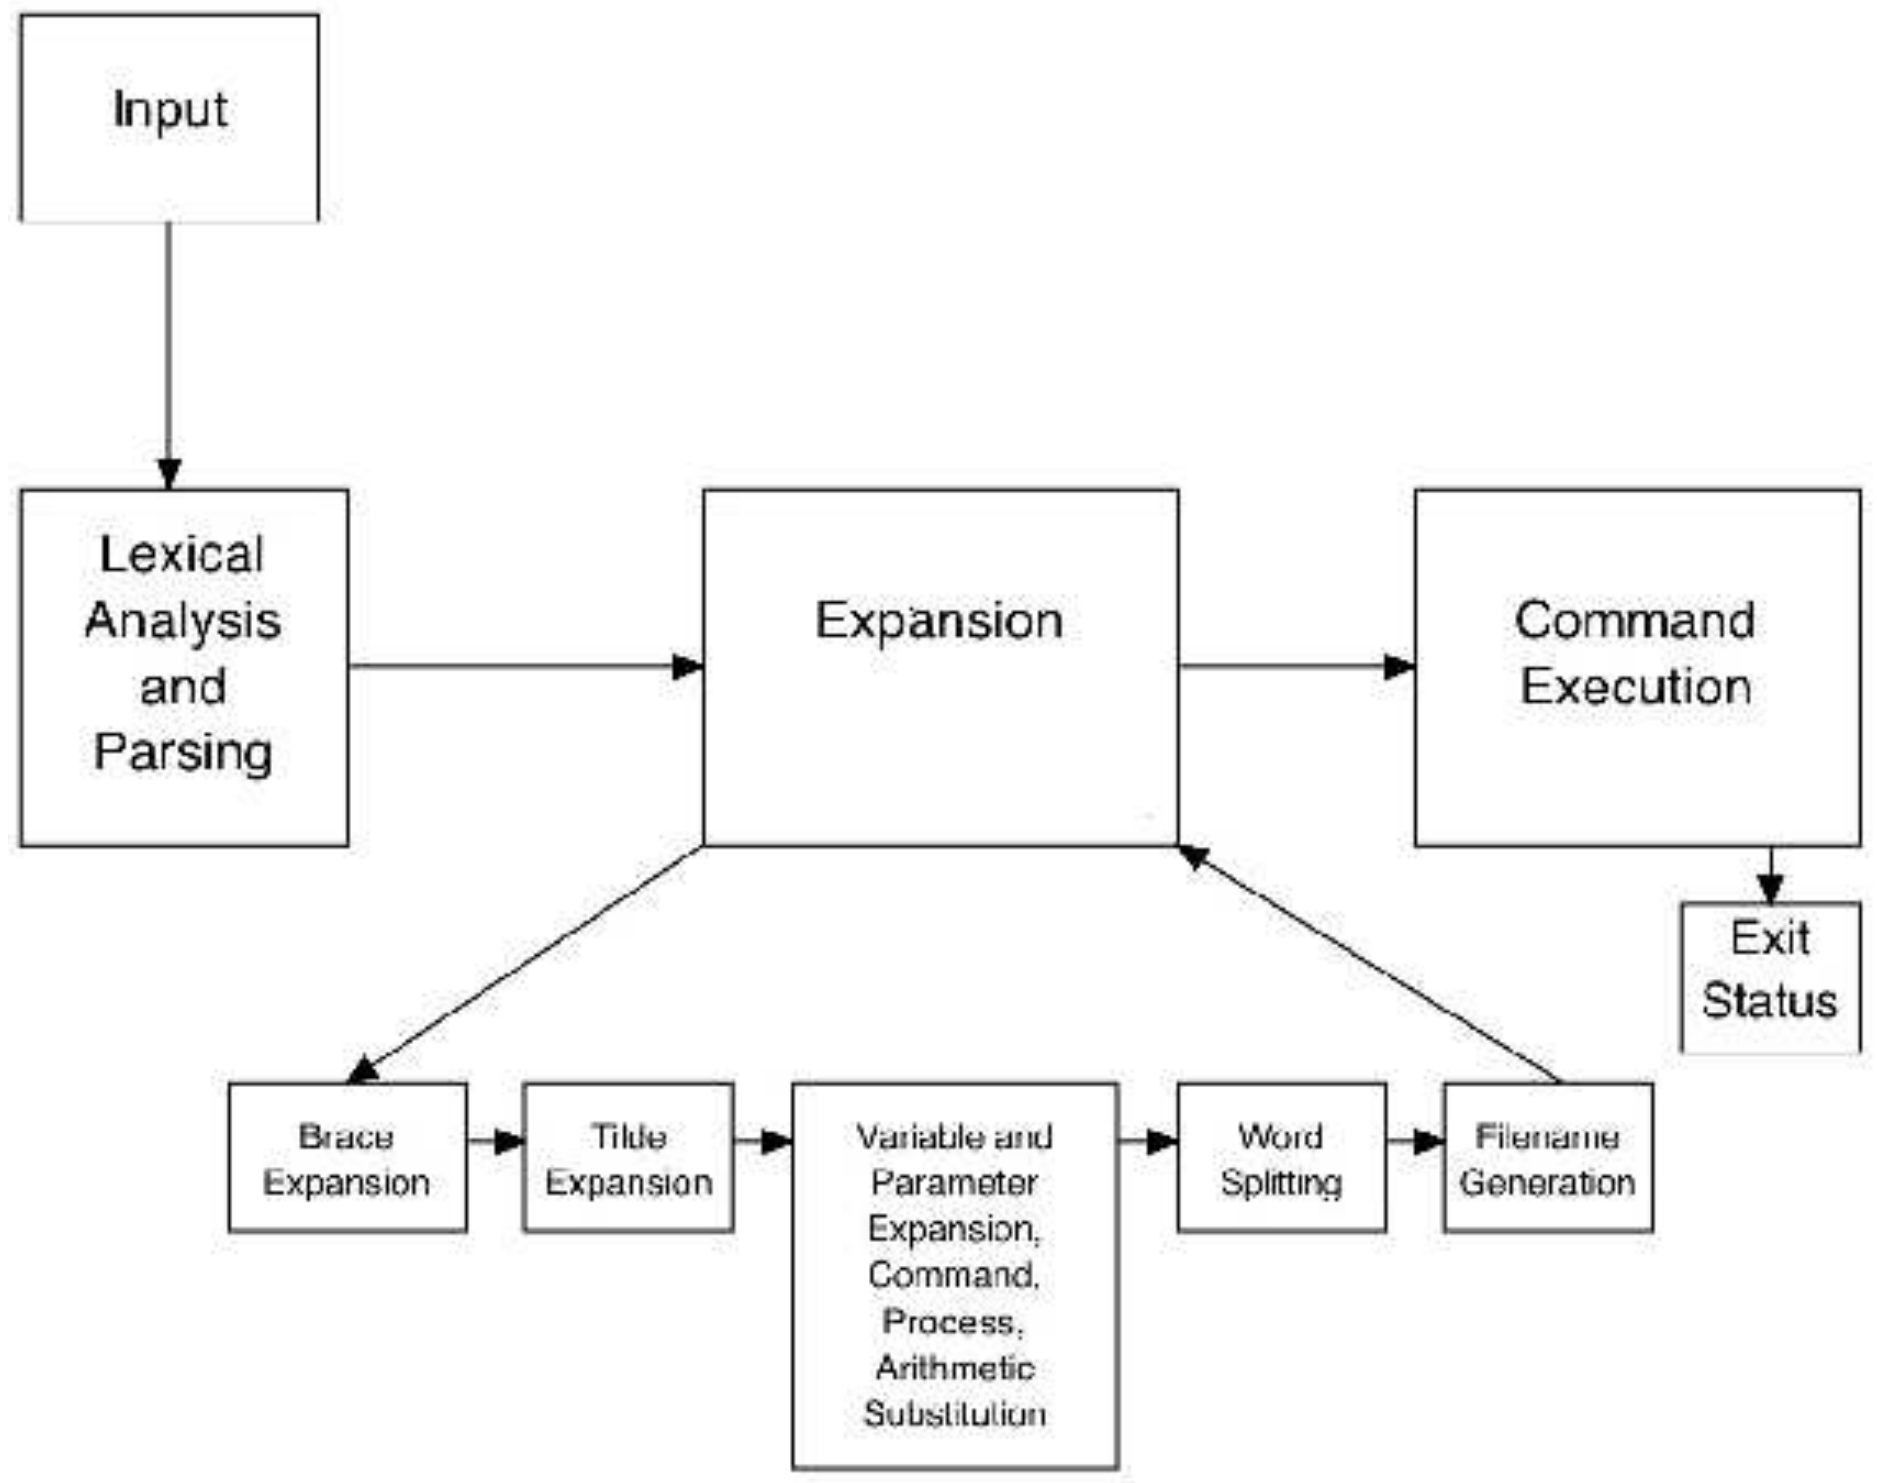
\includegraphics[width=0.7\textwidth]{bashArchitecture.png}
\end{center}

Диаграмма показывает поток данных между основными компонентами системы (в основном, Exit Status на самом деле компонентом системы не является, но я когда-то говорил, что неформальные диаграммы из квадратиков и стрелочек очень популярны и весьма полезны). Ввод (с консоли или из файла) поступает на вход лексическому и синтаксическому анализатору, далее последовательность слов, полученная парсером, отдаётся expansion-у, который на самом деле представляет собой конвейер, последовательно применяющий преобразования к последовательности слов. Сначала выполняется подстановка фигурных скобок, затем тильды, затем доллара, затем разделение на слова (после парсера, такие дела), затем раскрытие шаблонов. Дальше то, что получилось, подаётся на вход исполнялке команды, которая отвечает за перенаправление ввода-вывода, пайпы, группы процессов и т.д., в итоге получается результат выполнения команды в виде кода возврата.

Всё общение между компонентами выполняется с помощью структуры WORD\_DESC и различных контейнеров, содержащих эти структуры. Вот определение этой структуры:

\begin{minted}{c}
typedef struct word_desc {
    char *word; /* Zero terminated string. */
    int flags; /* Flags associated with this word. */
} WORD_DESC;
\end{minted}

А вот так, например, представляются аргументы команды:

\begin{minted}{c}
typedef struct word_list {
    struct word_list *next;
    WORD_DESC *word;
} WORD_LIST;
\end{minted}

\subsection{Ввод с консоли}

За ввод с консоли отвечает библиотека Readline, которая отвечает за редактирование командной строки и за хранение истории команд. Она устроена как цикл <<считать символ с клавиатуры --- найти команду, ему соответствующую --- исполнить её --- показать результаты>>. Символ считывается как 8-битный символ (в те времена, когда это писалось, юникода ещё не было) и используется как индекс в <<таблице диспетчеризации>>. В этой таблице может быть либо команда (например, <<перейти в начало строки>>), либо другая такая же таблица (это для поддержки сочетаний из нескольких символов), либо команда <<вывести считанный символ>>. Ещё есть макросы (которые просто вставляют во входной поток символы). Все выводимые символы хранятся в буфере редактирования, а когда надо вывести результат на экран, Readline хитро рассчитывает минимальный набор команд управления курсором, который преобразует текущую отображаемую на экране строку в желаемую. Все внутренние данные хранятся в виде 8-битных символов, но Readline знает (теперь) про юникод и умеет его корректно отображать и корректно считать позиции для многобайтовых символов.

Readline может быть расширена добавлением произвольных функций в таблицу диспетчеризации, и Bash этим пользуется, добавляя более 30 своих команд (например, автодополнение).

\subsection{Синтаксический разбор}

Readline возвращает просто строку, введённую пользователем. Первое, что с ней делается --- лексический анализ, то есть, в случае с Bash-ем, разделение по словам и их идентификация. С последним дела обстоят довольно плохо, потому что смысл последовательности символов сильно зависит от контекста, так что лексер и парсер должны тесно общаться друг с другом, чтобы разбирать, например, вот такой ужас:

\begin{minted}{sh}
for for in for; do for=for; done; echo $for
\end{minted}

Эта команда, кстати, вполне корректна и выведет на экран <<for>>.

Bash --- один из немногих шеллов, написаный на lex + bison, о чём, впрочем, автор несколько сожалеет, говоря, что ручная реализация рекурсивным спуском сильно упростила бы дело. Оригинальная грамматика шелла Борна, которую Bash пытается поддерживать, никому не известна, есть грамматика (контекстно-зависимая), стандартизованная POSIX, её-то и реализует Bash (так что грамматика Bash таки известна и документирована).

Интересно, что подстановка alias-ов выполняется лексером. Правда, для этого парсер сообщает ему, разрешена ли в данный момент подстановка. Лексер же отвечает за кавычки и бэкслеш.

Дополнительные проблемы создаёт подстановка результата выполнения команды и программируемое автодополнение, где тоже могут выполняться произвольные команды прямо в процессе разбора другой команды. Для поддержки таких вещей парсер умеет сохранять своё состояние и корректно восстанавливать его после разбора и исполнения <<подкоманды>>.

Результат работы парсера --- одна команда (которая в случае сложных команд типа for может содержать подкоманды), которая передаётся модулю, отвечающему за подстановки.

\subsection{Подстановки}

Подстановки (expansions) работают на уровне слов и могут порождать новые слова и списки слов. Они могут быть довольно сложными, например,

\begin{minted}{sh}
${parameter:-word}
\end{minted}

раскрывается в \textit{parameter}, если он установлен, и в \textit{word}, если нет. А

\begin{minted}{sh}
pre{one,two,three}post
\end{minted}

раскрывается в 

\begin{minted}{sh}
preonepost pretwopost prethreepost
\end{minted}

Ещё бывает подстановка тильды и арифметическая подстановка. Все они выполняются по порядку, то есть подстановщики организованы во что-то вроде конвейера.

Результат подстановки снова разбивается на слова (при этом это делает код, видимо, отличный от лексера). После разбиения происходит замена шаблонов --- каждое слово интерпретируется как потенциальный шаблон и пытается сопоставиться с файлом в файловой системе.

\subsection{Исполнение команд}

Команды бывают встроенными (которые модифицируют состояние самого шелла, например, cd) и внешними, которые сами отдельные программы (например, cat). Ещё бывают сложные команды --- if, for и т.д.

Каждая команда позволяет перенаправлять свой ввод и вывод (да, даже в for можно направить входной поток из пайпа). Самое сложное в реализации перенаправления --- это следить за тем, когда его нужно отменить. Встроенные и внешние команды работают с точки зрения пользователя одинаково, поэтому наивная реализация перенаправления вывода встроенной команды перенаправила бы вывод всего шелла. При этом Bash ещё и следит за файловыми дескрипторами, которые участвуют в редиректе, создавая новые или используя старые при необходимости.

Встроенные команды реализованы как сишные функции, принимающие список слов как аргументы, и работают как <<обычные>> команды, только без запуска отдельного процесса. Единственная тонкость в том, что некоторые команды принимают как аргумент присваивания (например, export), они обрабатывают присваивание по-особому (для этого используются флаги в WORD\_DESC). Обычные присваивания (которые не в export или declare) реализованы на самом деле тоже как команды, но парсятся и обрабатываются немного по-особому. Если присваивание стоит перед обычной командой, то оно передаётся команде и действует до её завершения, если присваивание одно на строке, оно действует на весь шелл. 

Внешние команды перед запуском ищутся в файловой системе, при этом шелл смотрит на PATH. Но если в имени команды есть слеши, то не ищет, а исполняет как есть. При этом единожды найдённая команда запоминается в хеш-таблице и дальше сначала ищется в ней. Если команда не нашлась, Bash вызывает функцию, которую можно переопределить, и многие дистрибутивы это делают, предлагая поставить нужный пакет с командой.

Ещё есть некоторые хитрости с управлением процессами, в которых исполняются команды. Есть режим foreground, в котором шелл ждёт завершения процесса с командой, есть background, где шелл запускает команду и тут же читает следующую. При этом Bash умеет переводить команду из одного режима в другой, для чего там есть понятие <<Job>>, как группа процессов, исполняющая команду. Например, пайпы собирают несколько процессов в один Job, который может быть отправлен в фон или в foreground целиком.

\subsection{Lessons learned}

Вот кратко вещи, на которые разработчик Bash Chet Ramey обратил внимание в ходе разработки.

\begin{itemize}
    \item Хорошие комментарии к коммитам со ссылками на багрепорты с шагами воспроизведения сильно облегчают жизнь.
    \item Хороший набор тестов --- тоже, Bash имеет тысячи тестов, покрывающие практически всю неинтерактивную функциональность.
    \item Сильно помогли стандарты, как внешние на функциональность шелла, так и внутренние на код.
    \item Хорошая пользовательская документация важна.
    \item Переиспользование сильно экономит время.
\end{itemize}

\subsection{Как обстоят дела на самом деле}

Товарищи из университета Южной Калифорнии исследовали <<настоящую>> архитектуру Bash с целью получить <<базовую>> архитектуру, по которой можно было бы оценивать эффективность различных инструментов автоматического восстановления архитектуры. Один аспирант 80 часов копался в исходниках, после чего отправил результаты автору и тот ещё высказал свои соображения. В итоге получилась вот такая структура системы:

\begin{center}
    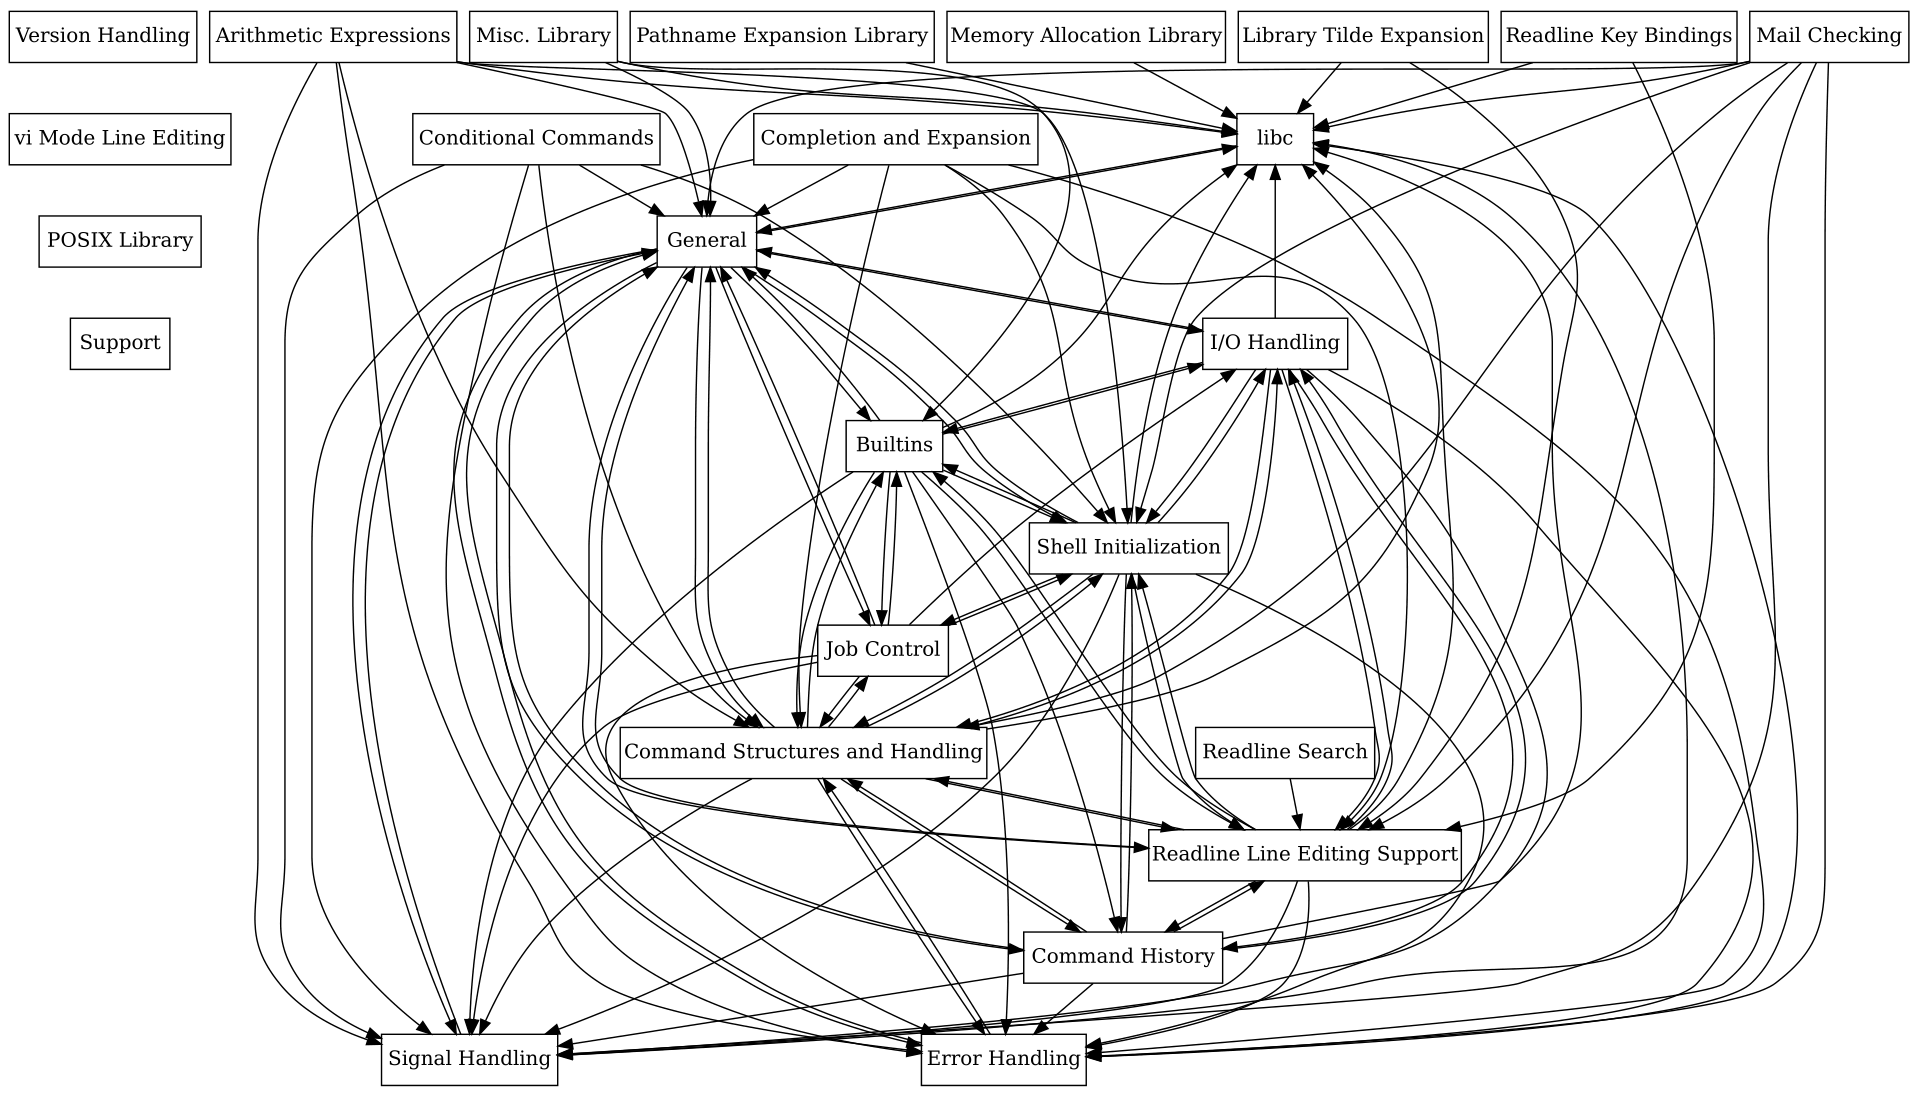
\includegraphics[width=\textwidth]{bashRealArchitecture.png}
\end{center}

Видно, что зависимостей в коде больше, чем на картинке с концептуальной архитектурой и поток данных на структурной диаграмме совершенно неочевиден. Но некоторые схожести всё-таки есть, например, ввод-вывод реально выделяются в отдельный кластер компонентов.

Bash имеет размер порядка 70К строк кода, около 200 отдельных файлов. В ходе восстановления архитектуры было выделено 25 компонентов, из которых 16 относятся к ядру функциональности системы, 9 --- вспомогательные. Выяснилось, что структура папок практически не соответствует компонентам, только два компонента имеют свои отдельные папки в исходниках.

Вот автоматически восстановленная по исходникам архитектура системы, с компонентами и зависимостями:

\begin{center}
    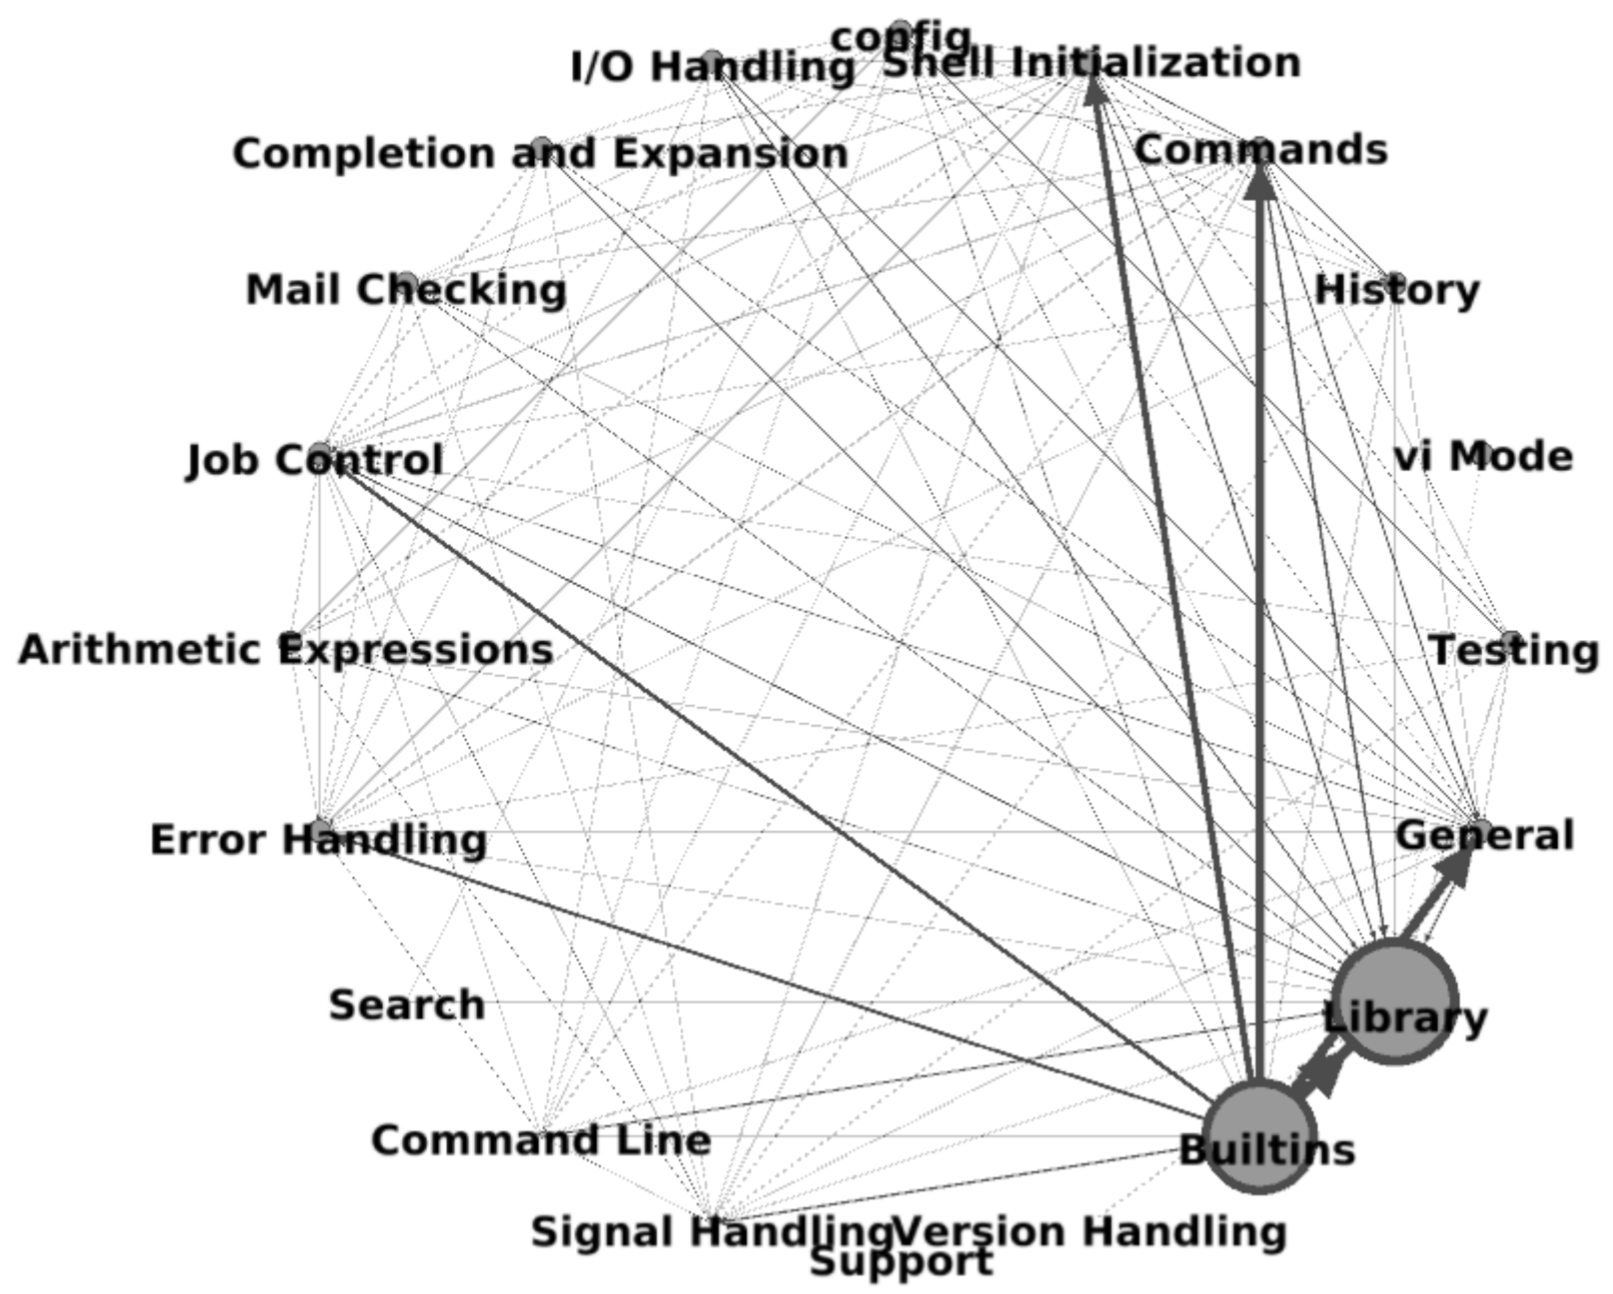
\includegraphics[width=0.7\textwidth]{bashAutomaticRecoveryArchitecture.png}
\end{center}

Сравните с исходной концептуальной архитектурой:

\begin{center}
    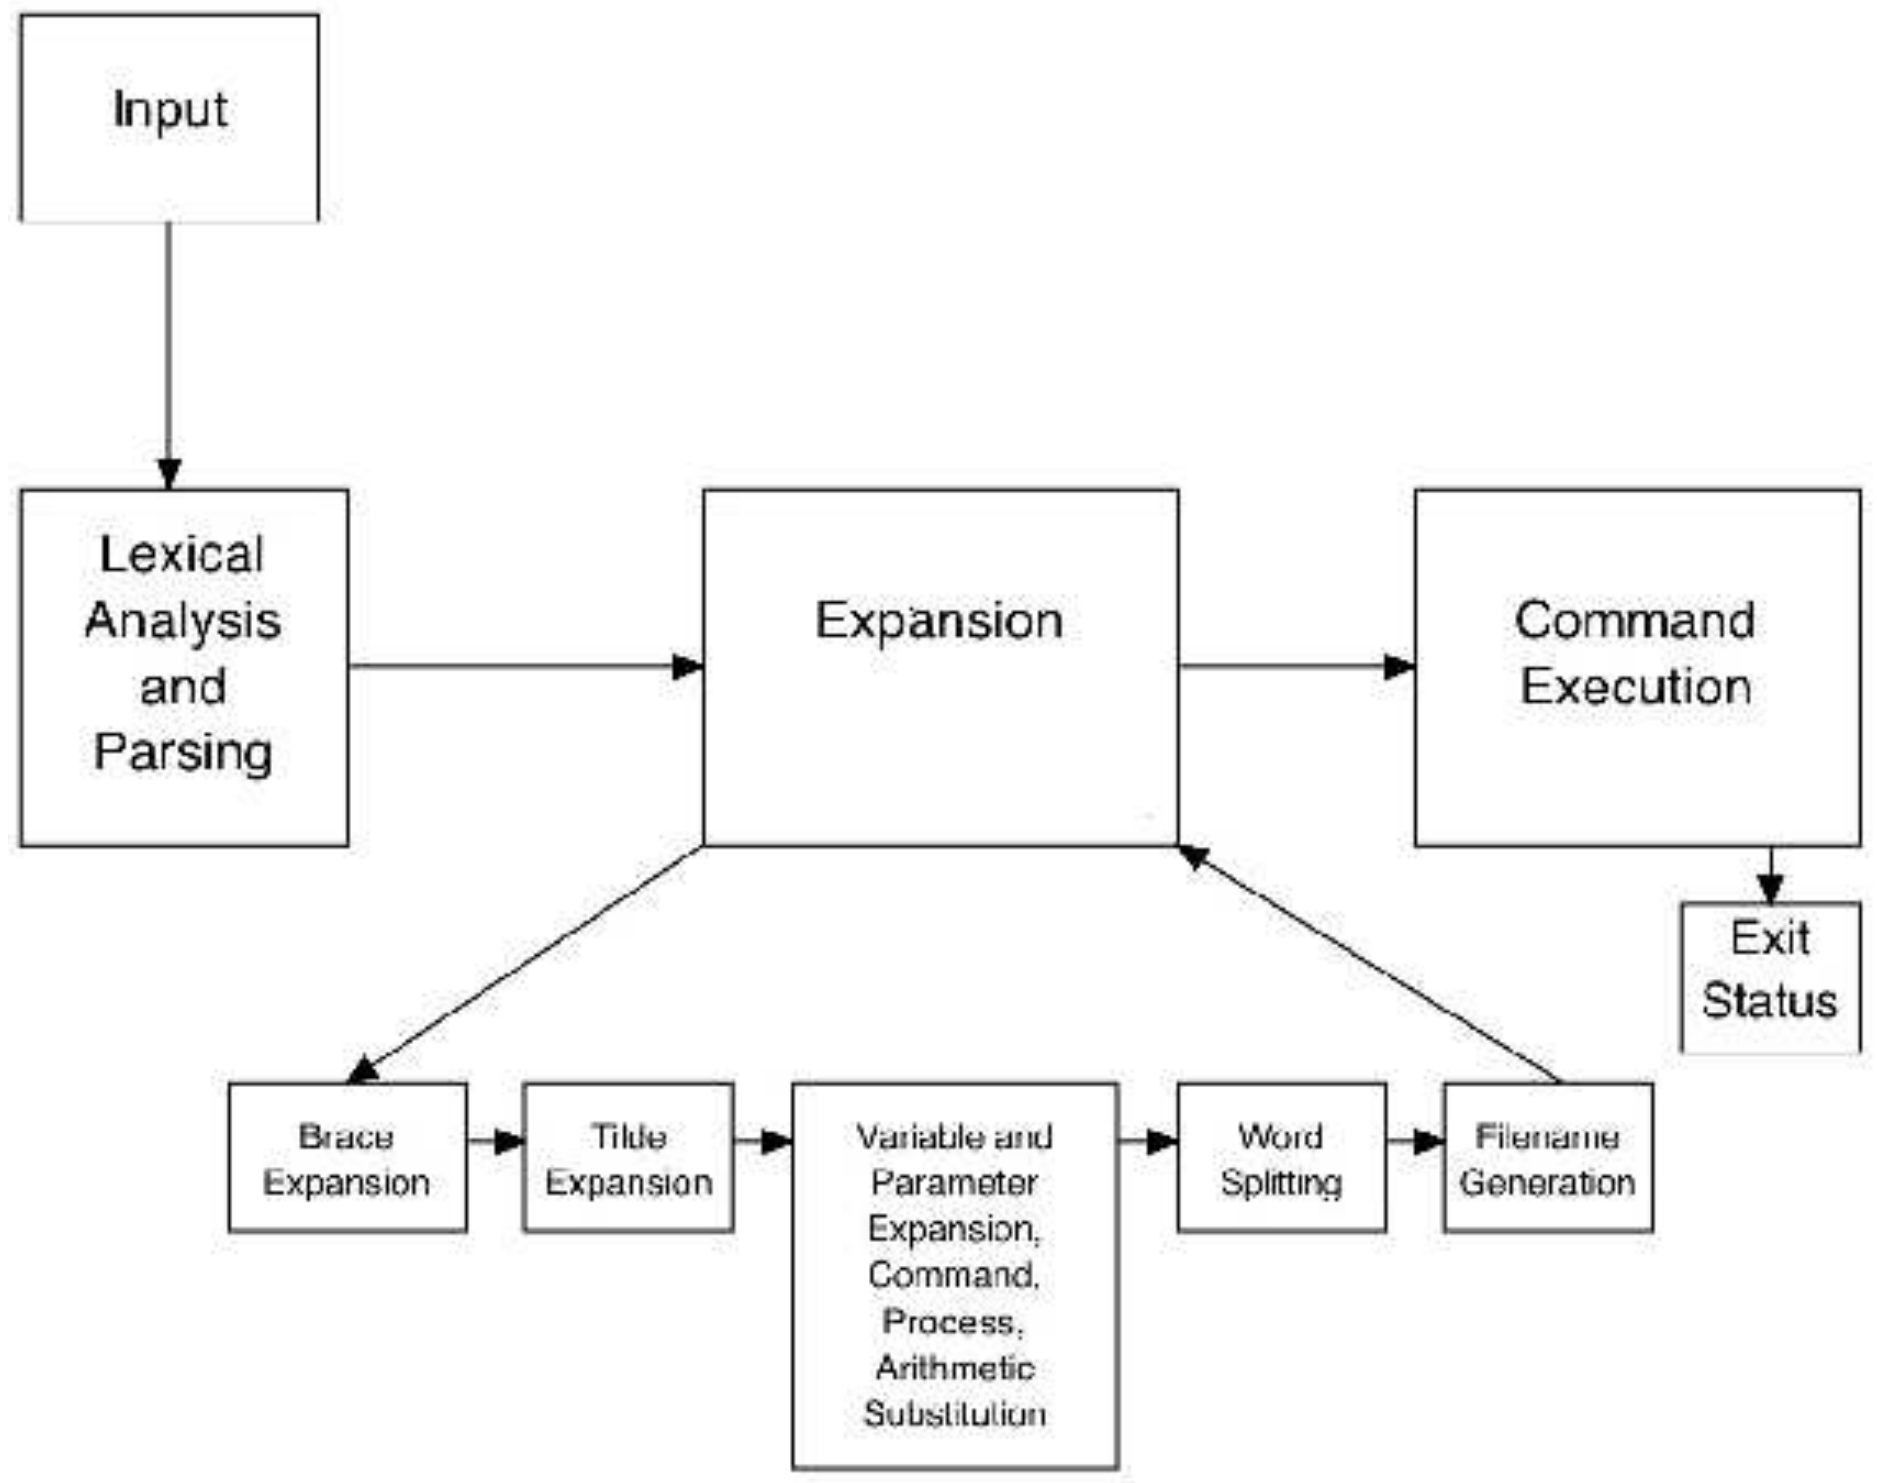
\includegraphics[width=0.6\textwidth]{bashArchitecture.png}
\end{center}

Это должно ещё раз проиллюстрировать мысль касательно архитектур реальных приложений --- есть архитектура как она проектировалась (prescriptive architecture), есть архитектура как она реализована в коде приложения (descriptive architecture), и в ходе эволюции приложения эти архитектуры становятся всё больше и больше непохожими друг на друга. Эти расхождения связаны с понятиями <<architectural drift>> (привнесение в архитектуру вещей, которых в исходной архитектуре на было, без нарушения принципов исходной архитектуры) и <<architectural erosion>> (привнесение в реализацию нарушений принципов исходной архитектуры). Для долгоживущих систем архитектурная эрозия становится довольно критичным фактором, приводящим к тому, что исходное разбиение на компоненты перестаёт быть валидным вообще. Bash в этом плане довольно показателен, поскольку ему много лет. Вот увеличенный вид компоненты управления Job-ами:

\begin{center}
    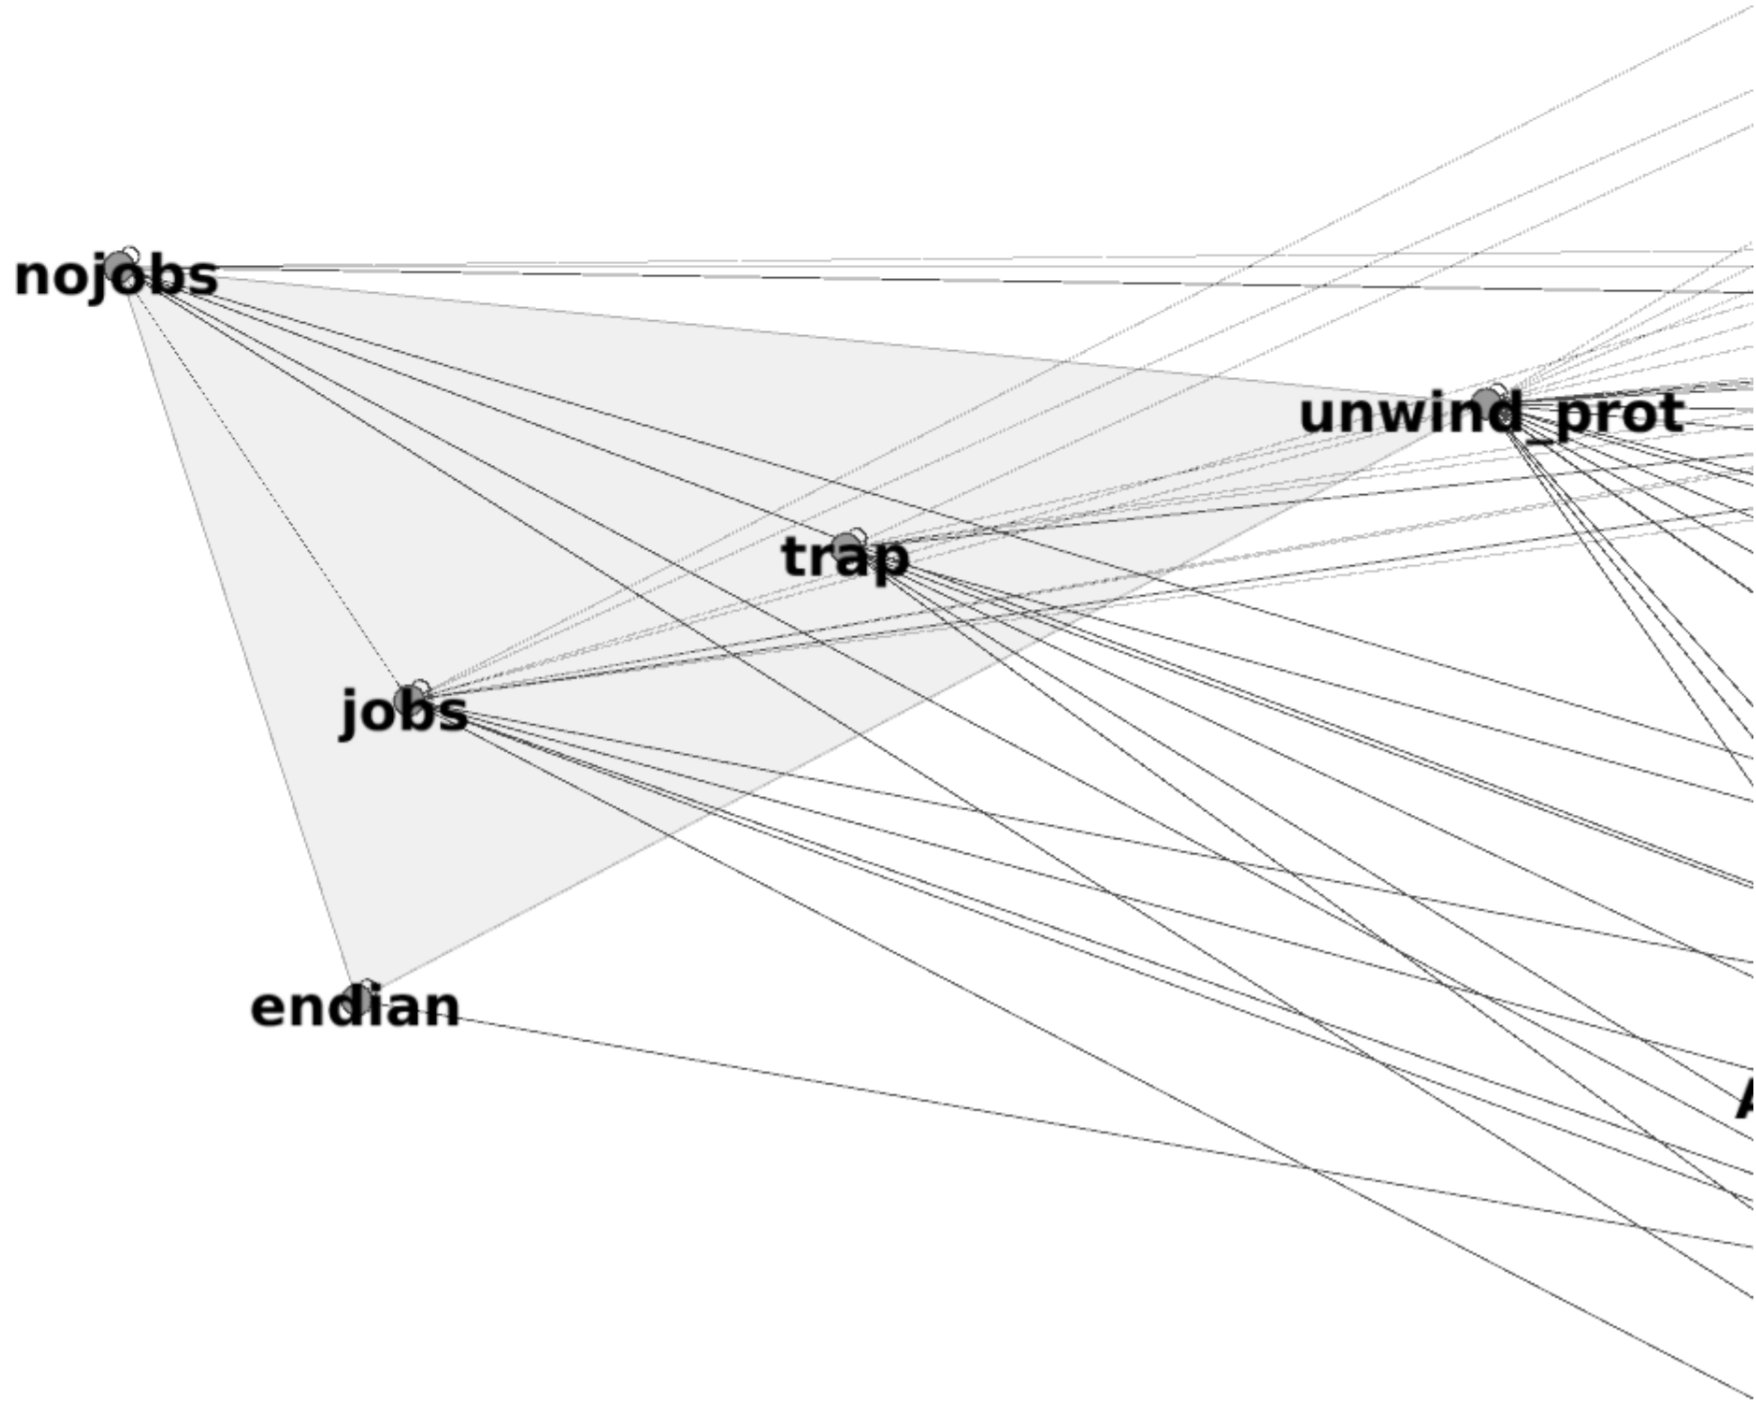
\includegraphics[width=0.6\textwidth]{bashJobControl.png}
\end{center}

Как видим, каждая сущность с этой компоненте больше связана с внешними сущностями, чем с сущностями внутри компоненты, то есть coupling очень высок, а cohesion, судя по всему, очень низок. С командами дела обстоят ещё хуже:

\begin{center}
    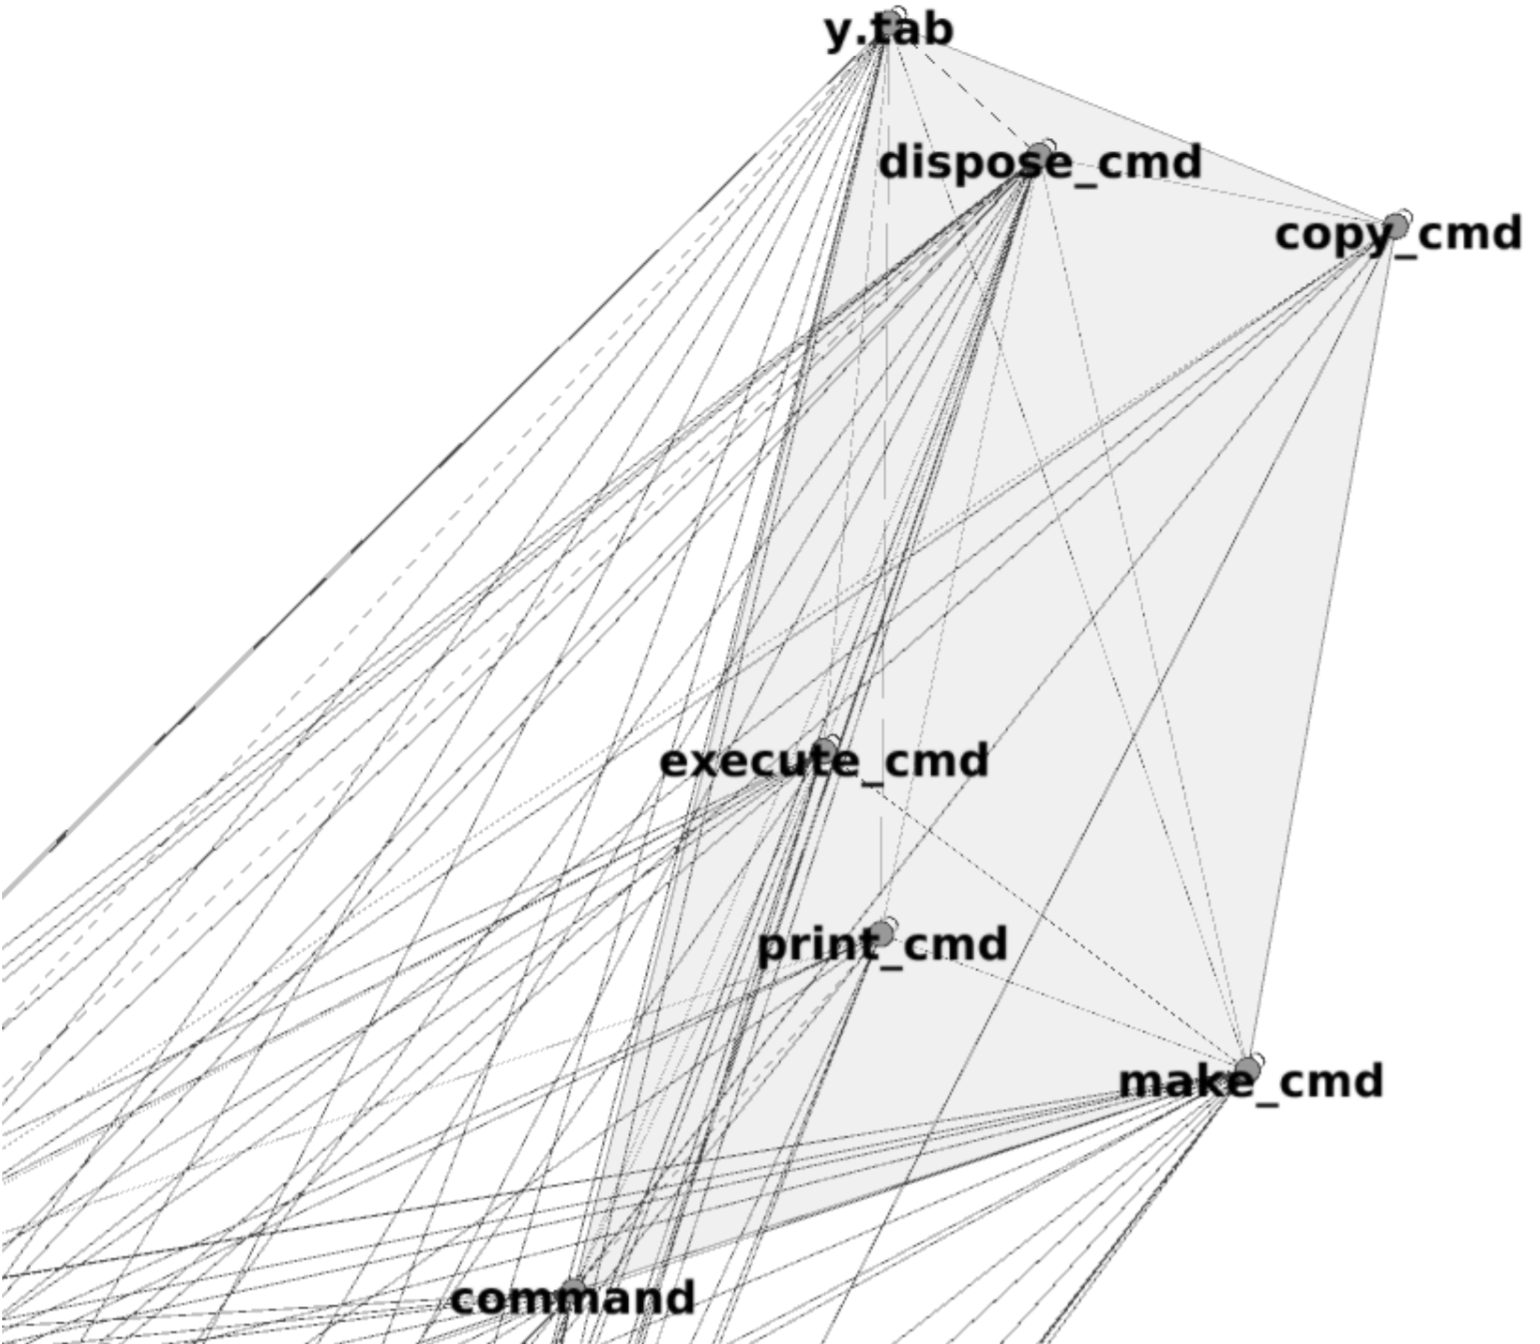
\includegraphics[width=0.6\textwidth]{bashCommands.png}
\end{center}

Собственно, поэтому важна архитектурная документация и нелишне наличие архитектора, который следил бы за тем, чтобы код и документация не очень расходились. Иначе приложение быстро превратится в гигантский ком кода, где всё зависит от всего и ломается при любом изменении.

\section{Git}

\subsection{Ключевые требования}

Git, как известно, распределённая система контроля версий. Появился он в результате грустной истории с ядром Linux --- оно некоторое время хранилось в проприетарной распределённой системе BitKeeper (2000 год, кстати, одна из первых), но потом разработчики ядра что-то не поделили с компанией-производителем (BitMover), и им пригрозили отзывом лицензии. Линусу Торвальдсу пришлось срочно разрабатывать новую систему контроля версий (потому что ему не нравилась система CVS, в которой так же хранились исходники Linux в то время). Поначалу это был просто набор скриптов на bash для управления патчами, приходившими по почте. С самого начала основными требованиями к разработке были следующие.

\begin{itemize}
    \item Распределённая разработка с тысячей коммитеров --- так же, как в BitKeeper и не так, как в CVS, должны были быть поддержаны процессы, при которых каждый участники может работать у себя локально, не мешая ничьей работе и сам определяя, когда его часть готова к публикации. Для большого проекта с открытым исходным кодом, надо которым работают тысячи никому ничего не должных энтузиастов, это необходимо.
    \item Защита от порчи исходников --- возможность отменить мердж, смерджиться вручную. Опять-таки, тысячи энтузиастов, которые никому ничего не должны, и половина из которых вообще толком программировать не умеет.
    \item Высокая скорость работы --- речь идёт о сотнях тысяч коммитов всё-таки.
\end{itemize}

Несколько иронично то, что BitKeeper сам в 2016 году стал опенсорсным, и при этом не то чтобы очень популярен. Никогда не ссорьтесь с opensource-сообществом по поводу лицензий на ПО.

\subsection{Представление репозитория}

Когда мы набираем \mintinline{text}|git init|, создаётся папка \mintinline{text}|.git|, где лежит вся информация гитового репозитория. Она имеет следующую структуру:

\begin{itemize}
    \item \textbf{HEAD} --- ссылка на текущую ветку, которую зачекаутили в рабочей папке;
    \item \textbf{index} --- staging area, то место, где формируется информация о текущем коммите;
    \item \textbf{config} --- конфигурационные опции гита для этого репозитория;
    \item \textbf{description} --- <<is only used by the GitWeb program, so don’t worry about it>> (c) Git Book;
    \item \textbf{hooks/} --- хук-скрипты (возможность исполнить произвольный код при каком-то действии типа коммита);
    \item \textbf{info/} --- тоже локальные настройки репозитория, сюда можно вписать игнорируемые файлы, которые вы не хотите писать в .gitignore, чтобы их не коммитить;
    \item \textbf{objects/} --- самое интересное, тут лежит собственно то, что хранится в репозитории;
    \item \textbf{refs/} --- тут лежат указатели на объекты из objects (ветки, как мы увидим в дальнейшем);
    \item \textbf{...} --- прочие штуки, которые появляются в процессе жизни репозитория и нам пока не интересны.
\end{itemize}

Гит вообще появился как набор утилит, которые позволяют быстро сделать систему контроля версий, а не как полноценная система контроля версий, так что у гита, помимо общеизвестных команд, есть и команды, позволяющие напрямую работать с репозиторием и делать с ним вручную ужасные вещи. Сам по себе репозиторий в гите --- это просто хеш-таблица, которая отображает SHA-1-хеш файла в содержимое файла, ничего более. Можно класть в неё объекты (даже не обязательно файлы), можно получать. Например, вот так:

\begin{minted}{bash}
$ git init test
Initialized empty Git repository in /tmp/test/.git/
$ cd test
$ find .git/objects
.git/objects
.git/objects/info
.git/objects/pack

$ echo 'test content' | git hash-object -w --stdin
d670460b4b4aece5915caf5c68d12f560a9fe3e4

$ find .git/objects -type f
.git/objects/d6/70460b4b4aece5915caf5c68d12f560a9fe3e4
\end{minted}

Создали пустой репозиторий, гит нам создал структуру папок \mintinline{bash}|.git/objects|, пока пустую. Командой \mintinline{text}|git hash-object| мы положили в репозиторий новый объект --- строчку \mintinline{bash}|'test content'|. Ключ \mintinline{bash}|-w| означает, что надо не просто посчитать хеш объекта, но и реально записать его на диск, ключ \mintinline{bash}|--stdin| означает, что содержимое объекта надо получить из входного потока, а не из файла. Вызов этой команды вернул нам SHA-1-хеш того, что получилось, и заодно создал файл на диске с содержимым, положив его в \mintinline{bash}|.git/objects|, в подпапку, называющуюся как первые два символа хеша, и в файл, называющийся как остальные 38 символов хеша.

Как достать то, что мы сохранили, обратно:
\begin{minted}{text}
$ git cat-file -p d670460b4b4aece5915caf5c68d12f560a9fe3e4
test content
\end{minted}

Команда \mintinline{bash}|git cat-file| показывает содержимое файла, ключ \mintinline{bash}|-p| говорит определить тип объекта и красиво показать его содержимое.

Уже можно сделать версионный контроль вручную с использованием рассмотренных команд (правда, для этого нам потребуется настоящий файл, версионировать строку, как в предыдущем примере, не интересно):

\begin{minted}{bash}
$ echo 'version 1' > test.txt
$ git hash-object -w test.txt
83baae61804e65cc73a7201a7252750c76066a30

$ echo 'version 2' > test.txt
$ git hash-object -w test.txt
1f7a7a472abf3dd9643fd615f6da379c4acb3e3a

$ find .git/objects -type f
.git/objects/1f/7a7a472abf3dd9643fd615f6da379c4acb3e3a
.git/objects/83/baae61804e65cc73a7201a7252750c76066a30
.git/objects/d6/70460b4b4aece5915caf5c68d12f560a9fe3e4

$ git cat-file -p 83baae61804e65cc73a7201a7252750c76066a30 > test.txt
$ cat test.txt
version 1

$ git cat-file -p 1f7a7a472abf3dd9643fd615f6da379c4acb3e3a > test.txt
$ cat test.txt
version 2
\end{minted}

Каждая новая версия в данном случае хранится как отдельный объект, но всему своё время.

Объект, кстати, называется <<blob>> (Binary Large OBject), и он хранит только данные, так что даже имя файла в нём не хранится, а, наверное, хотелось бы. За хранение имени файла, а также за хранение папок и вообще иерархии объектов отвечает объект <<tree>>. Например, вот так могло бы выглядеть дерево, на которое указывает коммит \mintinline{text}|master| в некотором репозитории (два файла и одно поддерево):

\begin{minted}{text}
$ git cat-file -p master^{tree}
100644 blob a906cb2a4a904a152e80877d4088654daad0c859      README
100644 blob 8f94139338f9404f26296befa88755fc2598c289      Rakefile
040000 tree 99f1a6d12cb4b6f19c8655fca46c3ecf317074e0      lib
\end{minted}

Синтаксис \mintinline{text}|master^{tree}| говорит, что надо отобразить master как tree-объект, а не как commit-объект. Вот так можно себе представить дерево, приведённое в примере:

\begin{center}
    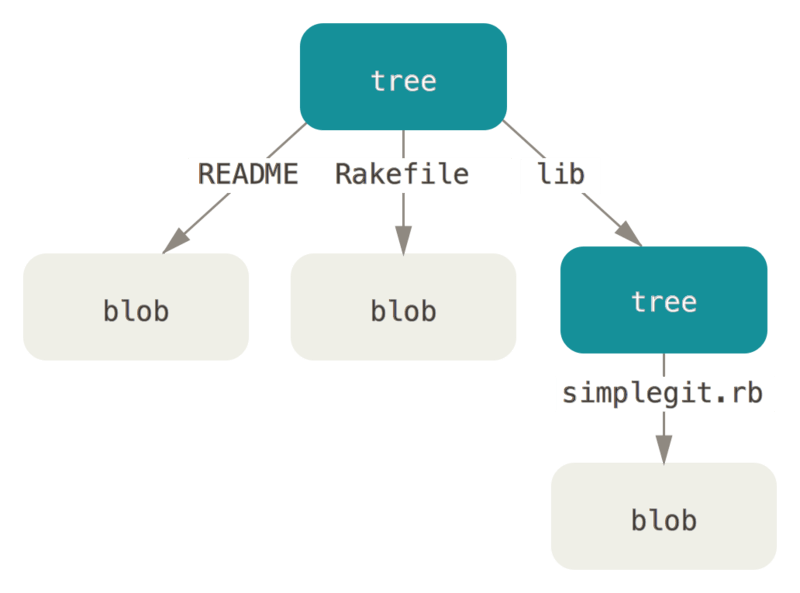
\includegraphics[width=0.5\textwidth]{gitTreeObject.png}
\end{center}

Вот примерная UML-диаграмма классов всех объектов, которые могут находиться в гитовом репозитории:
\begin{center}
    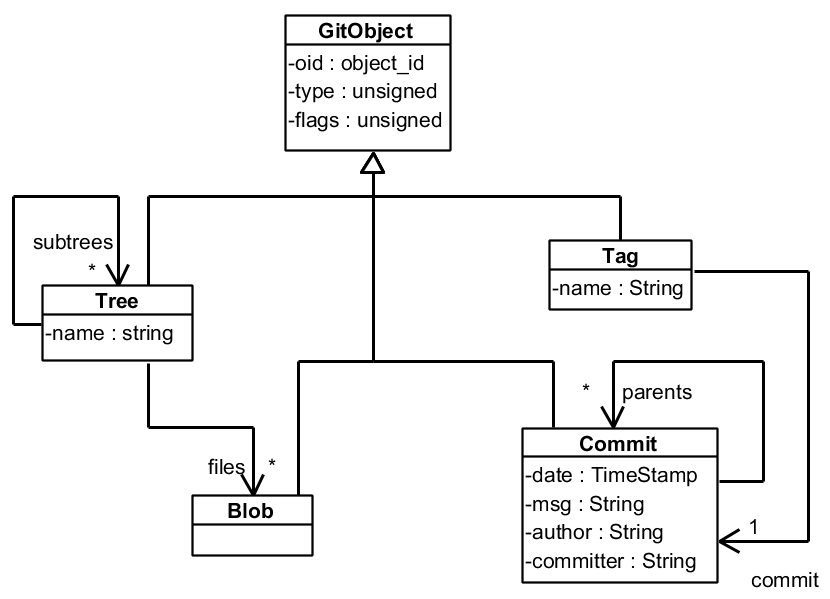
\includegraphics[width=0.7\textwidth]{gitDataStructure.png}
\end{center}

Все они являются объектами, поэтому имеют свой SHA-1-хеш, тип, который позволяет их отличить друг от друга, размер и данные. Blob и Tree мы уже видели, Tree содержит в себе поддеревья и Blob-ы. Осталось разобраться с коммитами и тэгами. 

Коммиты нужны для хранения метаинформации --- кто сделал изменение, когда и почему. Дерево ничего такого не хранит, в этом смысле оно напоминает узел файловой системы (в UNIX-подобных системах распространён термин inode), так что на объекты из дерева ссылаются коммит-объекты. Вот так это выглядит:
\begin{minted}{text}
$ echo 'first commit' | git commit-tree d8329f
fdf4fc3344e67ab068f836878b6c4951e3b15f3d

$ git cat-file -p fdf4fc3
tree d8329fc1cc938780ffdd9f94e0d364e0ea74f579
author Scott Chacon <schacon@gmail.com> 1243040974 -0700
committer Scott Chacon <schacon@gmail.com> 1243040974 -0700

first commit
\end{minted}

Ещё, что не показано на картинке, но тоже есть --- коммит хранит список коммитов-родителей, но вообще понятие <<родитель>> для коммита связано с ветками, поэтому про них чуть попозже. Вот, наверное, знакомая картинка про то, как коммиты можно представлять себе в виде указателей на узлы дерева в базе:

\begin{center}
    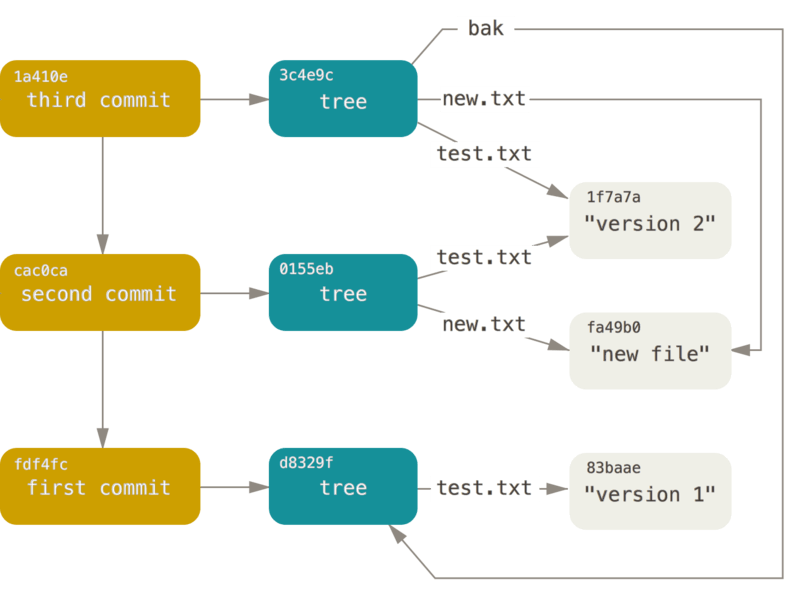
\includegraphics[width=0.7\textwidth]{gitCommitObjects.png}
\end{center}

Теперь у нас есть объекты, хранящие в себе содержимое файлов (blob-ы), объекты, хранящие в себе структуру файлов и их имена (tree-объекты), объекты, хранящие в себе информацию об истории модификаций первых двух видов объектов, и уже, в принципе, система контроля версий могла бы получиться. Но пользоваться ей было бы очень неудобно, потому что каждый объект идентифицируется только своим SHA-1-хешем, и чтобы делать что-нибудь содержательное, надо было бы эти хеши помнить. Чтобы с этим помочь, придуманы references. Reference --- это просто ссылка на коммит. Reference даже не объект, это просто файл, внутри которого лежит SHA-1-хеш объекта из базы. При этом reference-ы бывают двух типов --- head-ы и tag-и. Они хранятся в папке \mintinline{text}|.git/refs|, \mintinline{text}|.git/refs/heads| и \mintinline{text}|.git/refs/tags| соответственно. Мы можем сделать свою собственную ветку, создав сами такой файл:

\begin{minted}{text}
$ echo "1a410efbd13591db07496601ebc7a059dd55cfe9" > .git/refs/heads/master

$ git log --pretty=oneline master
1a410efbd13591db07496601ebc7a059dd55cfe9 third commit
cac0cab538b970a37ea1e769cbbde608743bc96d second commit
fdf4fc3344e67ab068f836878b6c4951e3b15f3d first commit
\end{minted}

Совсем вручную это делать можно, но не принято, есть команда \verb|git update-ref|, которая, во-первых, проверяет, что ref создаётся в правильной папке, во-вторых, заносит действие с reference в так называемый reflog, про который тоже чуть попозже, но вообще --- это штука, которая помнит, что происходило со ссылками и может помочь востановить случайно удалённую ветку. Традиционная картинка, поясняющая суть ссылок:

\begin{center}
    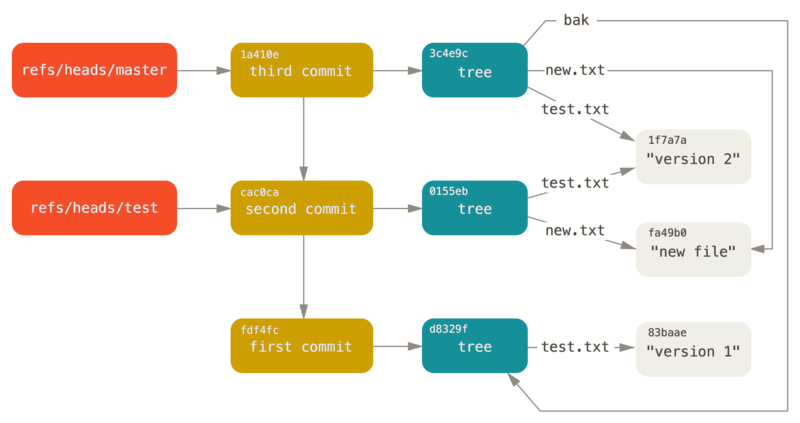
\includegraphics[width=0.9\textwidth]{gitRefs.png}
\end{center}

Среди всех ссылок выделяется самая главная, та, которая соответствует ветке, лежащей сейчас в рабочей копии. Она внезапно хранится не в \mintinline{text}|.git/refs|, а прямо в корне папки \mintinline{text}|.git|, в файле, который называется \mintinline{text}|HEAD|. Причём это даже не ссылка, а символическая ссылка, то есть ссылка на ссылку:

\begin{minted}{text}
$ cat .git/HEAD
ref: refs/heads/master

$ git symbolic-ref HEAD refs/heads/test
$ cat .git/HEAD
ref: refs/heads/test
\end{minted}

Команда \mintinline{text}|git symbolic-ref| нужна для <<вежливого>> обновления символической ссылки, которая проверяет корректность того, что происходит. Таким нехитрым образом можно переключаться между ветками, но обратите внимание, что \mintinline{text}|index| ничего про это не знает, так что файлы из старой ветки будут считаться добавленными к коммиту, потому что они были в её индексе и никто их оттуда не убрал. Так что \mintinline{text}|git checkout| всё-таки не только обновляет HEAD.

Последний из объектов, который надо рассмотреть --- это тэги. Тэг --- это просто указатель на коммит. Ну, на самом деле, не всё так просто, потому что мы видели его на диаграмме с объектами в базе, а reference --- не объект. Дело в том, что тэги бывают двух типов --- легковесные и аннотированные. Легковесный тэг --- это просто ссылка на коммит, которая никогда никем не двигается (её можно продвинуть вручную, но это плохо, поскольку тогда у людей, имеющих копии вашего репозитория, тэги могут начать не совпадать). Аннотированный тэг --- это уже полноценный объект, который указывает на коммит, и нужен он для того, чтобы иметь возможность добавить к тэгу разную метаинформацию типа автора, сообщения и даты.

Пример, как сделать вручную легковесный тэг:
\begin{minted}{text}
git update-ref refs/tags/v1.0 cac0cab538b970a37ea1e769cbbde608743bc96d
\end{minted}

А вот аннотированный тэг и как он хранится:
\begin{minted}{text}
$ git tag -a v1.1 1a410efbd13591db07496601ebc7a059dd55cfe9 -m 'test tag'

$ git cat-file -p 9585191f37f7b0fb9444f35a9bf50de191beadc2
object 1a410efbd13591db07496601ebc7a059dd55cfe9
type commit
tag v1.1
tagger Scott Chacon <schacon@gmail.com> Sat May 23 16:48:58 2009 -0700

test tag
\end{minted}

\subsection{Pack-файлы}

Казалось бы, теперь всё, но тут мы вспоминаем, что все объекты в репозитории всё ещё хранятся целиком, так что если у нас есть длиннющий исходник и мы в нём поменяли одну строчку, у нас получится два длиннющих исходника. Самое удивительное, что, в общем-то, в гите поначалу так и есть, репозиторий некоторое время просто раскопирует изменённые файлы. Естественно, файлы сжимаются zlib-ом, так что занимают чуть меньше места, чем могли бы, но всё равно, для системы контроля версий такая ситуация довольно странна. На помощь приходят pack-файлы:

\begin{minted}{text}
$ git gc
Counting objects: 18, done.
Delta compression using up to 8 threads.
Compressing objects: 100% (14/14), done.
Writing objects: 100% (18/18), done.
Total 18 (delta 3), reused 0 (delta 0)

$ find .git/objects -type f
.git/objects/bd/9dbf5aae1a3862dd1526723246b20206e5fc37
.git/objects/d6/70460b4b4aece5915caf5c68d12f560a9fe3e4
.git/objects/info/packs
.git/objects/pack/pack-978e03944f5c581011e6998cd0e9e30000905586.idx
.git/objects/pack/pack-978e03944f5c581011e6998cd0e9e30000905586.pack
\end{minted}

Тут мы выполнили команду \mintinline{text}|git gc| (Garbage Collect), в результате которой некоторые <<нормальные>> объекты удалились (на самом деле, все кроме <<висячих>>, то есть недостижимых по ссылкам) и появилось два файла: \mintinline{text}|.idx| и \mintinline{text}|.pack|. Второй файл содержит упакованными все наши объекты, и тут уже применяется дельта-компрессия, причём, что интересно, последняя версия файла хранится целиком, а предыдущие версии --- как дельты относительно более свежей версии, то есть как бы <<назад>> (что логично, скорее всего, последняя версия нужна чаще). Первый файл --- это оглавление для второго файла, именно его передают по сети, когда делается git push/git pull и локальный или удалённый гит пытается понять, какой информации у него нету. Вот так примерно это выглядит:

\begin{center}
    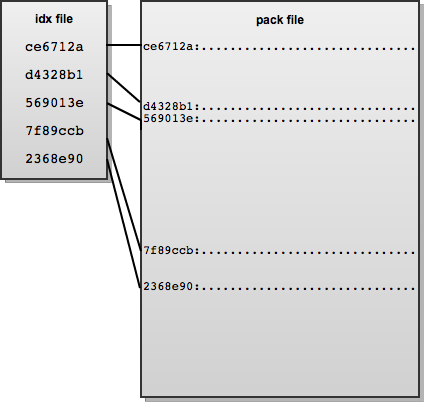
\includegraphics[width=0.6\textwidth]{gitPackFiles.png}
\end{center}

Упаковка объектов в .pack-файлы происходит, когда:
\begin{itemize}
    \item выполняется git push;
    \item слишком много <<свободных>> объектов (порядка 7000);
    \item вручную вызвана git gc.
\end{itemize}

Если pack-файл уже есть, то новые объекты могут упаковаться в новый файл, оставив старый неизменённым, а может произойти перепаковка и несколько .pack-файлов будут слиты в один (важно понимать, что .pack-файлов может быть несколько и вся работа с ними скрыта от пользователя системы контроля версий). Почему всё так хитро --- упаковка в .pack-файл требует пересчёта дельт и вообще очень трудоёмкая операция, так что делать её каждый коммит было бы очень раздражающе для пользователя. Есть ещё команда \mintinline{text}|git gc --auto|, которая проверяет, не надо ли запаковать объекты, она вызывается при каждом коммите и, как правило, ничего не делает, иногда всё-таки вызывая \mintinline{text}|git gc|. Внутрь pack-файла можно посмотреть командой \mintinline{text}|git verify-pack|, но это не то чтобы сильно полезно на практике, так что подробности в Git Book.

\subsection{Reflog}

Все нормальные команды гита записывают всё, что они делали с reference-ами, в файлы в папке \mintinline{text}|logs|, где, в частности, лежит лог того, что происходило со ссылкой \mintinline{text}|HEAD|, и его можно просмотреть командой \mintinline{text}|git reflog|:

\begin{minted}{text}
$ git reflog
1a410ef HEAD@{0}: reset: moving to 1a410ef
ab1afef HEAD@{1}: commit: modified repo.rb a bit
484a592 HEAD@{2}: commit: added repo.rb
\end{minted}

Или получить более подробную информацию командой \mintinline{text}|git log -g|:

\begin{minted}{text}
$ git log -g
commit 1a410efbd13591db07496601ebc7a059dd55cfe9
Reflog: HEAD@{0} (Scott Chacon <schacon@gmail.com>)
Reflog message: updating HEAD
Author: Scott Chacon <schacon@gmail.com>
Date:   Fri May 22 18:22:37 2009 -0700

    third commit
$ git branch recover-branch ab1afef
\end{minted}

Если мы случайно откатили ветку и потеряли тем самым какой-то нужный коммит, можно найти его в reflog-е, взять его хеш и сделать на него checkout.

А теперь как более капитально прострелить себе ногу. Шаг 1, удаляем ветку:

\begin{minted}{text}
$ git branch -D master
\end{minted}

Шаг второй, сносим все логи, чтобы нельзя было восстановить ветку по SHA-1-хешу последнего коммита, на который она указывала:

\begin{minted}{text}
$ rm -Rf .git/logs/
\end{minted}

Казалось бы, всё, репозиторий запорот и надо делать домашку заново? Нет, если база объектов на месте, можно воспользоваться командой \mintinline{text}|git fsck --full|, которая распечатает нам все висячие объекты вместе с их хешами:

\begin{minted}{text}
$ git fsck --full
Checking object directories: 100% (256/256), done.
Checking objects: 100% (18/18), done.
dangling blob d670460b4b4aece5915caf5c68d12f560a9fe3e4
dangling commit ab1afef80fac8e34258ff41fc1b867c702daa24b
dangling tree aea790b9a58f6cf6f2804eeac9f0abbe9631e4c9
dangling blob 7108f7ecb345ee9d0084193f147cdad4d2998293
\end{minted}

Теперь мы можем посмотреть на них командой \mintinline{text}|git cat-file -p|, выбрать тот, который больше всего похож на последний коммит той ветки, которую мы удалили, и восстановить ветку по его хешу: \mintinline{text}|git branch recover-branch ab1afef|. Ещё позитивно то, что Git не удалит даже <<висячие>> объекты несколько месяцев, если его явно не попросить, несмотря на то, как расшифровывается имя команды \mintinline{text}|git gc|, так что если вы потеряли ветку, то с большой вероятностью она всё ещё где-то есть и её можно восстановить.

\subsection{Lessons learned}

Поначалу некоторые команды были реализованы как шелл-скрипты, потому что так было быстрее. Однако это помешало, во-первых, интеграцию git со средами разработки, во-вторых, существенно усложнило портирование git на Windows. Что, в общем-то, не сильно расстроило Линуса Торвальдса и окологитовое сообщество середины 2000-х, но на самом деле негативно сказалось на внедрении git, поскольку крупные компании избегали пользоваться им из-за проблем с переносимостью. Впоследствии был реализован проект Git for Windows, где уже вся функциональность была реализована в виде разделяемой библиотеки, и дело пошло.

Ещё важный момент, проистекающий из изначального дизайна git как набора инструментов для управления патчами --- у него весьма хитрая система команд (<<plumbing>>, которым, в общем-то, никто не пользуется, и <<porcelain>>). Даже если не задумываться о том, что новички в git могут случайно нагуглить git cat-file и нескоро понять, что эти команды им знать не надо, набор команд сложноват и не то чтобы дружественен к начинающим пользователям. На первом курсе, чтобы научить студентов пользоваться git, требуется обычно две пары, плюс у них всё равно весь первый курс время от времени возникают проблемы, требующие некоторого вмешательства.

\section{Battle for Wesnoth}

Следующий пример архитектуры диаметрально противоположен консольным утилитам. Речь пойдёт про игру Battle for Wesnoth, пошаговую стратегию с открытым исходным кодом, один из относительно немногих подобных проектов, который реально играбелен, развивается более 15 лет и до сих пор жив, имеет 93\% позитивных отзывов (из более 2700) на Steam. При этом игра распространяется бесплатно и имеет порядка 4 миллионов скачиваний, включая скачивания со Steam и официального сайта. Разработка началась в 2003 году, игра написана на C++ и на данный момент имеет кодовую базу порядка 200000 строк кода, плюс порядка 250000 строк декларативного описания контента на их собственном предметно-ориентированном языке.

\subsection{Architectural Drivers}

Вся архитектура игры строится вокруг одного принципа --- доступности для новых разработчиков и авторов контента. Для некоммерческого open-source-проекта возможность привлекать сторонних авторов, быстро вводить их в курс дела и давать возможность создавать контент или править движок игры --- критична для выживания. Как обычно, речь идёт о проекте, где никто никому ничего не обязан, который живёт достаточно долго, чтобы несколько поколений maintainer-ов успели потерять интерес, где, в отличие от систем, рассмотренных ранее, большая часть интересующихся проектом людей --- скажем так, не очень зрелого возраста, и в подавляющем большинстве без технического образования.

Поэтому основными требованиями, легшими в основу архитектуры, стали:
\begin{itemize}
    \item возможность декларативно создавать контент (кампании, юниты, карты, сюжет и т.д.) на предельно простом предметно-ориентированном языке;
    \item использование широко распространённых библиотек, минимизация внешних зависимостей;
    \item простота кода, возможно, в ущерб технической красоте;
    \item кроссплатформенность.
\end{itemize}

\subsection{Высокоуровневая архитектура}

Диаграмма <<компонентов>> проекта представлена на рисунке:

\begin{center}
    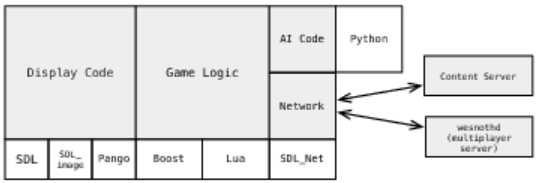
\includegraphics[width=0.5\textwidth]{wesnothArchitecture.png}
\end{center}

Опять-таки, диаграмма из квадратиков и стрелочек вместо формальных нотаций UML (чтобы не смущать юных кодеров). И, кстати, эта мутная картинка --- лучшее, что удалось найти про высокоуровневую архитектуру системы (и то в AOSA, не в каком-нибудь диздоке на сайте проекта, а вики на гитхабе у них вообще отсутствует). Это, на мой взгляд, несколько противоречит идее о быстром и простом введении новых разработчиков в проект, но увы.

Итак, на диаграмме белым выделены внешние библиотеки, серым --- то, что непосредственно относится к проекту. Стрелочками с основной игрой соединены отдельные программы:

\begin{itemize}
    \item wesnothd --- сервер для многопользовательской игры;
    \item content server --- репозиторий с кампаниями, картами и другим дополнительным контентом, с помощью которого прямо из игры можно качать расширения.
\end{itemize}

Ввод-вывод и отрисовка графики выполняются библиотекой SDL (Simple Directmedia Layer), очень известной в игровой индустрии. Она умеет работу с клавиатурой/мышью, отображение двумерной графики, звук, портирована на все нормальные и не вполне нормальные платформы (например, Android, так что SDL-приложения, скорее всего, даром запустятся там, но без тюнинга пользовательского интерфейса будут неиграбельны).

Boost используется как библиотека общего назначения, стандартная для практически любого проекта на C++, она обеспечивает кучу полезных вещей, которые постепенно перекочёвывают в стандартную библиотеку, но до C++11 программировать без Boost на плюсах было упражнением в мазохизме (если вы не использовали какие-то другие подобные библиотеки, типа Qt).

Pango + Cairo --- для отображения текста с учётом локализации, zlib --- стандарт де-факто, если надо что-нибудь архивировать, Lua и Python для скриптования, GNU gettext для интернационализации.

Сама система состоит из следующих компонентов.

\begin{itemize}
    \item Парсер и препроцессор WML (Wesnoth Markup Language) --- тот самый DSL, на котором описывается весь контент игры.
    \item Базовый ввод-вывод --- видео, звук, сеть поверх SDL.
    \item GUI --- виджеты пользовательского интерфейса (всякие кнопки, текстовые поля, полосы прокрутки и т.д.).
    \item Display module --- игровая сцена, юниты, анимация и т.д. Это не GUI, потому что отображение сцены всё-таки отдельная большая задача, большая часть специфичного для системы кода относится именно к игровой сцене.
    \item Модуль ИИ --- думаю, понятно (хотя, наверное в наше время стоит особо отметить, что в играх ИИ --- это не про нейросети).
    \item Поиск пути --- модуль для поддержки ИИ, содержит, помимо собственно, алгоритмов поиска пути, утилиты для работы с гексагональной доской, поскольку это тоже не очень тривиальная задача.
    \item Генератор карт --- не все карты рукодельные, есть и развитый механизм случайной генерации.
    \item Специализированные модули --- модуль титульного экрана, Storyline module (для проигрывания катсцен по ходу кампании), <<Play game>> module (управление основным игровым процессом).
\end{itemize}

\subsection{Wesnoth Markup Language}

Wesnoth Markup Language --- язык для описания контента. Изначально планировалось использовать XML-описания, но авторы решили ориентироваться на контентоделов, для которых даже HTML или Python кажутся сложными и породили следующее:

\begin{minted}{text}
[unit_type]
    id=Elvish Fighter
    name= _ "Elvish Fighter"
    image="units/elves-wood/fighter.png"
    hitpoints=33
    advances_to=Elvish Captain,Elvish Hero
    {LESS_NIMBLE_ELF}
    [attack]
        name=sword
        icon=attacks/sword-elven.png
        range=melee
        damage=5
    [/attack]
[/unit_type]
\end{minted}

В принципе, очень похоже на XML, но, как видно, атрибуты и дочерние тэги синтаксически не очень различаются, и атрибуты выглядят несколько более симпатично, чем в XML (хотя бы без лишних кавычек). К тому же, нет всяких неймспейсов и тэги выглядят менее <<агрессивно>>. Кроме того, есть препроцессор --- например, директива \mintinline{text}|{LESS_NIMBLE_ELF}| тут используется для подстановки стандартных для эльфов параметров.

Вообще, препроцессор довольно развитый, умеет в параметры макросов, условные операторы и т.п. Например,

\begin{minted}{c++}
#define GOLD EASY_AMOUNT NORMAL_AMOUNT HARD_AMOUNT
    #ifdef EASY
    gold={EASY_AMOUNT}
    #endif
    #ifdef NORMAL
    gold={NORMAL_AMOUNT}
    #endif
    #ifdef HARD
    gold={HARD_AMOUNT}
    #endif
#enddef
...
{GOLD 50 100 200}
\end{minted}

Тут описывается макрос с тремя параметрами, который в зависимости от настроек сложности кампании выбирает одно из трёх переданных ему значений. \mintinline{text}|{GOLD 50 100 200}| --- вызов макроса где-то в конфиге, который, видимо, даёт ИИ меньше денег, если игрок выбрал более лёгкий уровень сложности.

WML-описания контента разбиты по разным файлам, при загрузке уровня они все сливаются в один гигантский WML-документ, препроцессируются и загружаются в модель данных в программе. При этом при смене опций модель данных перепрепроцессируется и перезагружается заново (как раз из-за условных операторов в препроцессоре). Чтобы это не было убийственно для производительности (на некоторых машинах загрузка документа занимала до минуты), применяются всякие хаки на уровне препроцессора, например, определение своей переменной препроцессора для каждой кампании и \mintinline{c}{#ifdef}-ы, окружающие специфичный для кампании контент, чтобы даже не рассматривать его при загрузке других кампаний. Кроме того, WML-документы кешируются.

В качестве хранилища данных о юнитах используется класс unit\_type. Для представления конкретного юнита на поле боя используется класс unit, имеющий ссылку на соответствующий unit\_type. unit\_type-ы грузятся при загрузки WML в глобальную таблицу типов юнитов (это что-то вроде стиля <<Knowledge Layer>>, unit\_type декларативно описывает, что можно делать с юнитами, unit представляет сущность <<операционного>> уровня). 

ИИ смотрит на unit и unit\_type и выбирает поведение юнита исходя из флагов, прописанных в WML, и его текущего состояния. В WML нет никакой возможности описать логику действий юнита (даже декларативно), всё, что можно сделать, это ставить флаги. Например, <<skirmisher>> скажет ИИ и логике игры, что юнит может свободно перемещаться вблизи от юнитов врага, а не заканчивать ход, как обычные юниты. Это осознанное решение, поскольку задание поведения юнита в императивном стиле, безусловно, серьёзно расширило бы возможности контентоделов, но существенно усложнило бы описание контента. Поэтому, исходя из architectural drivers, от этой идеи отказались. Всё поведение ИИ и все возможности юнитов должны быть поддержаны в коде.

Такая же идея стоит за классом attack\_type, описывающем возможные типы атак. Есть фиксированный набор видов атаки и эффектов, поддерживаемых движком (например, дальняя атака, атака ближнего боя, магическая атака), можно из базовых атрибутов собирать атаку конкретного вида оружия (например, атака мечом --- 4 попытки нанести урон от 1 до 8 холодным оружием) и давать атаки юнитам (может, несколько), при этом игрок может выбрать, какую атаку использовать в конкретной ситуации (например, лучники эффективны против юнитов чисто ближнего боя, потому что последние не могут ответить на дальнюю атаку).

Кроме того, для большей <<ролеплейности>> игрового процесса, каждому юниту при создании назначаются случайные особенности. Например, сильный юнит сильнее атакует в ближнем бою, умный юнит требует меньше опыта для прокачки. Да, каждый юнит имеет дерево прокачки c преобразованием в другой тип юнита (то самое \mintinline{text}{advances_to=Elvish Captain,Elvish Hero} в WML). При этом у каждого юнита есть инвентарь, куда можно добавить вещи, которые ещё как-то модифицируют параметры юнита. Если вспомнить, что речь идёт о стратегии, а не о RPG, звучит неплохо.

\subsection{Мультиплеер}

Архитектура многопользовательской игры заслуживает отдельного упоминания. Сервер работает по протоколу TCP/IP и реализован максимально просто: есть начальное состояние игры, которое при создании игры рассылается всем подключённым клиентам, и пользовательские команды. При выполнении хода игрока команды сериализуются и рассылаются всем подключённым клиентам, и при этом сохраняются в логе игры на сервере. Клиенты проигрывают команды, тем поддерживая синхронность изменений игрового мира. При этом новый клиент может подключиться прямо в процессе игры, ему пошлют начальное состояние и все команды из лога, так что он сможет восстановить текущее состояние игры. Это же даёт бесплатно возможность просматривать повтор игры.

Сервер просто пересылает команды между клиентами, никакой игровой логики на сервере нет. Нет и никакой защиты от читов, и это тоже осознанное архитектурное решение --- авторы решили, что в Wesnoth не должны устраивать соревновательные матчи, все игры должны быть дружескими и для удовольствия, а не для победы. Потому посылать некорректные с точки зрения игровой логики команды можно, сервер не возражает, но ожидается, что психически здоровые пользователи не будут этого делать. Единственное, что проверяется при подключении --- версии клиентов, если они не сойдутся, то проигрывание команд может привести к разным результатам, так что клиенту с неправильной версией отказывают в подключении.

\subsection{Lessons Learned}

Итого, результатами разработки WML и выбранной стратегии максимального упрощения стало то, что сейчас кода на WML больше, чем кода на C++ (порядка 250К строк кода WML против 200К кода на C++). К игре сделали сотни пользовательских кампаний, и бесчисленное количество других ресурсов. Репозиторий имеет более 77 тысяч коммитов, более 200 контрибьюторов, более 600 форков. Так что можно считать, что цели проекта (выжить и развиваться в условиях, когда типичному пользователю 12 лет) полностью достигнуты. 

Сами разработчики в AOSA в секции Lessons Learned рассказывают больше про то, как крут их проект а не про то, чему они научились. Единственная самокритика заключается в том, что WML кажется самим же разработчикам весьма убогим и неэффективным. Однако же успех проекта показал, что технически неправильное решение изобрести велосипед оказалось правильным в плане возможностей по привлечению авторов контента. В целом, авторы делают вывод, что задача сделать и контент, и код доступными для модификации приходящими в проект людьми, особенно без богатого опыта разработки, очень сложна. Я бы сказал, в плане движка игры они и не пытались особо, но может, это и к лучшему, чтобы уж совсем тупые script kiddies не отвлекали своими пуллреквестами нормальных разработчиков.

\end{document}
